 %% Version 4.3.2, 25 August 2014
%
%%%%%%%%%%%%%%%%%%%%%%%%%%%%%%%%%%%%%%%%%%%%%%%%%%%%%%%%%%%%%%%%%%%%%%%%%%%%%%%%%%%%%%%%%%%%%%%%%%%%%%%%%%%%%%%%%%%%%%%%%%%%%%%%%%%%%%%%
% PREAMBLE
%%%%%%%%%%%%%%%%%%%%%%%%%%%%%%%%%%%%%%%%%%%%%%%%%%%%%%%%%%%%%%%%%%%%%

%% Start with one of the following:
% DOUBLE-SPACED VERSION FOR SUBMISSION TO THE AMS
% \documentclass{ametsoc}

% TWO-COLUMN JOURNAL PAGE LAYOUT---FOR AUTHOR USE ONLY
\documentclass[twocol]{ametsoc}

%%%%%%%%%%%%%%%%%%%%%%%%%%%%%%%%
%%% To be entered only if twocol option is used

\journal{jcli}


%  Please choose a journal abbreviation to use above from the following list:
% 
%   jamc     (Journal of Applied Meteorology and Climatology)
%   jtech     (Journal of Atmospheric and Oceanic Technology)
%   jhm      (Journal of Hydrometeorology)
%   jpo     (Journal of Physical Oceanography)
%   jas      (Journal of Atmospheric Sciences)	
%   jcli      (Journal of Climate)
%   mwr      (Monthly Weather Review)
%   wcas      (Weather, Climate, and Society)
%   waf       (Weather and Forecasting)
%   bams (Bulletin of the American Meteorological Society)
%   ei    (Earth Interactions)

%%%%%%%%%%%%%%%%%%%%%%%%%%%%%%%%
%Citations should be of the form ``author year''  not ``author, year''
\bibpunct{(}{)}{;}{a}{}{,}

%%%%%%%%%%%%%%%%%%%%%%%%%%%%%%%%%%%%%%%%%%%%%%%%%%%%%%%%%%%%%%%%%%
%% Matt's added packages: (idk if I'm allowed to do this in my submission but I think so)
\usepackage{amsmath}
\usepackage{graphicx}
\usepackage[colorinlistoftodos]{todonotes} %% For comments that will show in the pdf
\usepackage{gensymb} %%for degree symbols mainly


%% Delete before submission:
%\usepackage{refcheck}

% For table:
% Please add the following required packages to your document preamble:
\usepackage{booktabs}
\usepackage{multirow}
\usepackage[normalem]{ulem}
\useunder{\uline}{\ul}{}
\usepackage{lscape} %%for landscape table
\usepackage{makecell} %to force newline in table cell
% \usepackage{longtable} %%for table wrap to next page

%%%%%%%%%%%%%%%%%%%%%%%%%%%%%%%%

%%% To be entered by author:

%% May use \\ to break lines in title:

%% \title{Trends in Ice Storms throughout the Great Lakes Region}
\title{Recent Changes in Ice Storms and Freezing Rain\\ throughout the Great Lakes Region}

%%% Enter authors' names, as you see in this example:
%%% Use \correspondingauthor{} and \thanks{Current Affiliation:...}
%%% immediately following the appropriate author.
%%%
%%% Note that the \correspondingauthor{} command is NECESSARY.
%%% The \thanks{} commands are OPTIONAL.

    %\authors{Author One\correspondingauthor{Author One, 
    % American Meteorological Society, 
    % 45 Beacon St., Boston, MA 02108.}
% and Author Two\thanks{Current affiliation: American Meteorological Society, 
    % 45 Beacon St., Boston, MA 02108.}}

\authors{Matthew C. Irish\correspondingauthor{Matt Irish, National Renewable Energy Laboratory, 15013 Denver West Parkway, Golden, CO 80401.}\thanks{Majority of work done while at the Department of Climate and Spaces and Engineering, University of Michigan, Ann Arbor, Michigan.}} 

\affiliation{ National Renewable Energy Laboratory, Golden, Colorado}

\email{mairish@umich.edu}

%% If appropriate, add additional authors, different affiliations:
    %\extraauthor{Extra Author}
    %\extraaffil{Affiliation, City, State/Province, Country}
\extraauthor{Richard B. Rood}
\extraaffil{Department of Climate and Space Sciences and Engineering, University of Michigan, Ann Arbor, Michigan}
\extraauthor{William J. Baule}
\extraaffil{Department of Geography, Environment, and Spatial Sciences, Michigan State University, East Lansing, Michigan}

%%%%%%%%%%%%%%%%%%%%%%%%%%%%%%%%%%%%%%%%%%%%%%%%%%%%%%%%%%%%%%%%%%%%%
% ABSTRACT[RBR3]
% Abstracts should not exceed 250 words in length!
\abstract{Despite the expensive and deadly impacts that ice storms have upon major population centers in the Great Lakes region of North America and the region's status as a center of freezing rain activity, little research has been devoted to better understanding trends in the spatial and temporal distribution of these events, especially in regard to anthropogenic climate change. This work extends the most recent Great Lakes freezing rain climatology (1976--1990) to analyze trends and their underlying dynamics by making use of observations made through 2014. To isolate regional trends and determine changes in the synoptic-scale processes driving them, a k-means objective clustering algorithm is applied to pressure anomaly maps and records of freezing rain observations to create three archetypal synoptic weather patterns associated with ice storms. A northward shift in freezing rain incidence is evident across the Great Lakes on an annual basis, accompanied by a seasonal trend toward winter, with more frequent freezing rain occurrence in January and fewer incidences of freezing rain in the fall and spring months of November and March. The largest regional trend was a **\% decrease (+1.9 hrs yr$^{-1}$ decade$^{-1}$) in hourly freezing rain observations throughout Pennsylvania, upstate New York, and the St. Lawrence Lowlands of Canada since 1976. The northernmost region included in the study, the southern expanse of the Canadian Shield, saw an increase of **\% (-**hours decade$^{-1}$), and in the low-lying Atlantic Coastal Plain of Long Island and Manhattan an increase of **\% (-1.3 hrs yr$^{-1}$ decade$^{-1}$) was observed. The low-pressure centers of each of the three synoptic weather patterns migrated northward roughly ~200-500 km between the first and second half of the 1979--2014 period, consistent with warmer temperatures and northward-moving extratropical cyclone tracks. Observed trends have generally matched and outpaced model projections.}

\begin{document}
%% Necessary!
\maketitle
%%%%%%%%%%%%%%%%%%%%%%%%%%%%%%%%%%%%%%%%%%%%%%%%%%%%%%%%%%%%%%%%%%%%%
% MAIN BODY OF PAPER
%%%%%%%%%%%%%%%%%%%%%%%%%%%%%%%%%%%%%%%%%%%%%%%%%%%%%%%%%%%%%%%%%%%%%
%
\section{Introduction}
Freezing rain occurs when rain that has been supercooled to below 0\degree C without having crystallized into ice pellets (also known as sleet) instantaneously freezes to form glaze ice upon striking a surface that is also below 0\degree C. This can happen via either of two microphysical processes: the "classical formation process" or "melting process" where ice crystals falling through a shallow (usually roughly 1 km), above-freezing air mass melt into supercooled rain before freezing instantaneously on any sub-freezing surface, and the "warm rain" process where this supercooled rain instead results from cloud droplets coalescing by random collision (without having originated as ice crystals higher in the troposphere). \citet{rauber2000relative} provides a host of references describing these two processes and explores their relative contributions to freezing rain incidence in the United States. The melting process often leads to freezing drizzle, which is not considered in this work since it is characterized by small droplets that are not thought to contribute much to glaze ice accretion. When the thickness of glaze ice causes widespread damage or exceeds a subjectively-defined thickness, commonly 0.25 inches [0.64 cm] on a flat surface (as defined by the National Weather Service), we refer to such a weather event as an ice storm \citep{nwsglossary}.

\subsection{Impacts of ice storms}
Although the mild temperatures and winds present during ice storms often leave such events neglected in discussions of extreme weather, the economic damages and human health impacts of accumulated glaze ice from freezing rain often compare with those of tornadoes, severe thunderstorms, and occasionally, hurricanes \citep{lott2006tracking}. In North America, ice storms occur most frequently in the upper U.S. Midwest, northeastern U.S., and southeastern Canada (collectively referred to here as the Great Lakes region), as well as in the Columbia River Basin of the Pacific Northwest, where temperature inversions are frequent \citep{changnon2003temporal, bernstein2000regional}. In the northeastern region of the U.S. adjacent to the St. Lawrence river valley, freezing rain was observed at some point during roughly 5--7 days each year throughout the middle of the twentieth century \citep{changnon2003temporal}. In roughly the same period (1919--1969), the probability of at least one ice storm (defined using the 0.64 cm threshold set by the National Weather Service) occurring each year in any given location averaged across Pennsylvania, New York, and New England was 88\% \citep{tattelman1973estimated}. 

Over the past several decades, single storms in the northeastern U.S. and the Great Lakes have caused billions of dollars in damages and taken dozens of lives, with an average cost of \$193 million and 26 deaths attributed to ice and sleet events each year in the latter half of the twentieth century \citep{lott2006tracking, changnon2006severe, ncei2019storm}. Ground and air transportation networks are subject to delays and fatal accidents even under mild icing conditions on roads and runways. Icing also presents a danger aloft: when aircraft fly through supercooled raindrops, reductions in lift and control of aerodynamic surfaces from glaze ice accretion have caused crashes on rare occasion \citep{bernstein2000freezing}. Injuries and deaths are common from falling trees, slips and falls, downed power lines, and carbon monoxide inhalation due to the use of poorly ventilated generators during power outages \citep{daley2000outbreak}. Power line and pole failure under excessive ice thickness is the most intuitive cause of power outages during ice storms, but blackouts can also result from vehicular accidents involving utility poles, phase-to-phase faults from line galloping or lines that rebound after melting ice falls off, and arc flash across heavily-iced insulators at towers and switching stations. Power system impacts are not limited to failures of transmission and distribution infrastructure: generating capacity is sometimes reduced during and after ice storms when wind turbines are curtailed (i.e. forced offline) due to excessive blade icing. This can last for days and even up to several consecutive weeks in regions highly susceptible to ice storms as well as rime ice and hoarfrost accumulation \citep{davis2014forecast}. The New England Independent System Operator, for example, noted anecdotally that blade icing is a primary reason for wind curtailment in its balancing authority area (i.e. the region of the power system it oversees) \citep{bird2014wind}. As development of new wind energy projects accelerates, this makes understanding recent trends in freezing rain occurrence particularly important for financial projections, power system reliability and resilience planning studies, and safety considerations during the siting process concerning ice throw. Most system operators do not formally collect information on wind curtailment or its causes, however, so there has been no quantitative analysis published to-date on the system reliability impacts of such shutdowns or their costs to generators and ratepayers.

Damage to natural systems by the presence of glaze ice has also been documented, mainly in regard to forest management and damage to the vegetation that wildlife relies on for food and shelter \citep{pellikka2000modelling,proulx2001relationship}. Experience also suggests that floods due to ice jams on partially thawed rivers and lakes can be worsened due to increased ice accretion from freezing rain, although we were unable to find any study evaluating such a link. 

When the impacts discussed above are coincident with those of severe snowstorms and thunderstorms, as they often are, the damage done by each additional extreme weather phenomenon intensifies and entire regions of North America can be temporarily paralyzed. A power system failure can shut down the trains, trams, and buses that rely on it. When roads are icy, emergency response times can increase just as those services are in highest demand, as can the amount of time it takes to repair damaged infrastructure. Recovery efforts can be further impaired when wireless telecommunication networks are fractured due to the structural failure of lattice towers and guy wires. Conceptualizing ice storms as a risk multiplier and considering their high degree of spatial variability makes studying trends in freezing rain occurrence at a detailed spatial scale of great interest if we are to cleverly allocate resources toward climate change adaptation.

\subsection{Human-caused changes in the climatology of ice storms}
Ice storms often form narrow, predominantly latitudinal bands just north of the surface-level 0\degree C isotherm across the regions they affect, bounded by snow to the north and rain to the south. These bands have been expected to shift northward as the climate continues to warm \citep{cheng2011possible,lambert2011simulated}. It is intuitive how this would occur as the 0\degree C isotherm migrates toward Earth's poles, but this notion is complicated by the fact that freezing rain is triggered under several different synoptic conditions and its occurrence is heavily influenced by local topography and proximity to large bodies of water like the Great Lakes and the Atlantic Ocean. It is further obfuscated when we consider that any trend in freezing rain frequency is defined by changes not just in the phase of precipitation but also in the overall amount of precipitation, which could either reinforce or counteract the former influence. 

If we are then to try and discern likely impacts on society by thinking in terms of changes in glaze ice accretion due to ice storms, the task becomes even more complicated: the local duration of freezing precipitation, the intensity of the rainfall throughout the event, and other factors such as wind and temperature heavily influence ice accretion, and all may be affected by human interference in the climate system.  As \citet{lubchenco2012extreme} noted while serving as head administrators of the National Oceanic and Atmospheric Administration (NOAA), ice storms rank at the bottom amongst extreme weather phenomena in regard to our knowledge of the physical factors influencing their formation, reliable data concerning their climatology, and our understanding of any role humans may have on those factors now and in the future.

Looking forward into the twenty-first century, \citet{lambert2011simulated} applied a precipitation-typing algorithm to climate model simulations of a moderate warming scenario for 2081--2100 and found that freezing rain events are expected to shift poleward with modest increases in freezing rain incidence to the north and substantial decreases to the south. \citet{cheng2011possible} came to similar conclusions using statistical downscaling and synoptic precipitation typing of climate projections to predict substantial increases in freezing rain frequency throughout southeastern Canada in January and February with a progressively greater effect from south to north. Decreases were projected in the fall and warmer winter months. The two studies, however, focused on slightly different regions and came to differing conclusions about whether seasonal increases overwhelm the decreases on an annually-averaged basis. Taking a different approach, a thought experiment by \citet{klima2015ice} calculated changes in expected freezing rain frequencies by applying a precipitation typing algorithm to historical soundings modified by a uniform warming across the entire vertical profile. Under such simulated conditions, freezing rain frequencies were expected to decrease throughout the year in the southeastern and central U.S. but shift toward winter in the area extending northward from roughly Michigan's Upper Peninsula across to New York's Adirondacks and Maine. Most recently, a study using the Canadian Regional Climate Model to project freezing rain, ice pellets, and mixed precipitation for 2070 to 2099 using climate scenario RCP 8.5 predicted annual decreases in such precipitation types for the St. Lawrence River valley and northeastern U.S \citep{matte2018mixed}. This was mostly due to a projected decrease in long duration events of more than six hours. 

\citet{groisman2016recent} provided the first evidence showing temporal changes in freezing rain distributions in recent years. Their analysis focused on North America and Europe as a whole and the analysis of trends used least squares linear regression to conclude that there have been annual increases in freezing rain frequency in the arctic region of North America and decreases in the southeastern U.S. Most ice storms and the greatest impacts on humans, however, are concentrated between those two extremes, in the mid-latitudes. We also contend below that the use of a parametric trend test like linear least squares makes assumptions that are poor for time series of freezing rain observations.

The most recent freezing rain climatology to focus on the Great Lakes region was published in 2000, made use of observations from 1976 to 1990 \citep{cortinas2000climatology}, and did not analyze trends. Our purpose here is to build upon that climatology by investigating trends in the frequency, duration, and intensity of freezing rain events through 2014 and then to identify any underlying changes in the weather systems that bring them about. 

That analysis of underlying dynamics draws from the results of \citet{rauber2001synoptic}, who carried out a manual classification of 411 freezing rain and freezing drizzle events occurring east of the Rocky Mountains from 1970 to 1994 (all the ice storms recorded in the National Centers for Environmental Information \textit{Storm Data} publication for that time period) and identified seven dominant weather patterns. These classifications were later consolidated by \citet{erfani2012automated} into three patterns by applying a k-means objective typing algorithm and statistical analysis to reanalysis maps of surface level pressure anomalies and partial thicknesses. \citet{erfani2012automated} used the same storms identified by Rauber for validation of the methodology and analyzed the significance of the patterns using wind speed and precipitation statistics from NCEP data. We extend this methodology by using a similar synoptic weather typing algorithm that includes representation of surface pressure anomalies, the warm layer aloft, and the locations of freezing rain observations to assess changes over time in each weather pattern and in the number of storms of each type that occurred.

These changes in climate dynamics are compared with the projections referenced above as well as those previously linked to human emissions of greenhouse gases in the scientific literature to investigate how the observed trends fit into the larger frame of anthropogenic climate change.


\section{Data}
The study area was defined similarly to that of \citet{cortinas2000climatology}, but reaching further eastward, from 96\degree W to 72\degree W and 38\degree N to 50\degree N. Data were analyzed for all U.S. states that border the Great Lakes---Illinois, Indiana, Michigan, Minnesota, New York, Ohio, Pennsylvania, and Wisconsin---plus Iowa and the Canadian provinces of Ontario and Quebec.

\subsection{Weather station observations}
Since estimates of freezing rain incidence are included in several well-known reanalyses, a climatology could be created based only upon one of these products, but a few factors would make such an analysis unreliable. One regional reanalysis with high vertical resolution, for example, the North American Regional Reanalysis (NARR), provides estimates of freezing rain incidence using the precipitation typing algorithm developed by \citet{baldwin1993development} for the NCEP Eta Model, which drives NARR. A direct comparison of NARR's precipitation type flags with station observations was carried out in a case study of a 1990 event that affected the South-Central U.S. by \citet{blunden2011138}, indicating that NARR estimates are unreliable predictors of station observations. This was attributed in part to the fact that NARR reports only one precipitation type at each grid cell in every three-hourly product. Models originally developed to identify winter precipitation types for numerical weather prediction (such as those described by \citet{cortinas2002probabilistic} and \citet{mullens2017multialgorithm}) have been applied to reanalysis outputs with mixed results. A recent example is the model described by \citet{kamarainen2017method}, which compares vertical profiles of relative humidity and temperature with regionally-calibrated threshold values to identify likely precipitation type. The model achieved a 36-year spatially-averaged correlation with weather station observations of 0.93 over all of Europe, but comparing results at individual grid cells containing weather stations with freezing rain observations, the model yielded a mean correlation of only 0.44. This exemplifies the drawback of such approaches: modeling each of the two formation processes leading to freezing rain and discerning them from other precipitation types, ice pellets in particular, is difficult even with a high vertical resolution \citep{reeves2014sources}. In addition, the influence of topography and proximity to bodies of water occurs at a highly localized scale that may not be properly reflected when averaged into a grid cell. Considering all these limitations, temporally consistent direct observations from weather stations offer the most reliable means of assessing the true distribution of freezing rain.

The primary data for this investigation are freezing rain observations from hourly surface weather reports that are part of the Integrated Surface Database (ISD) maintained by the National Centers for Environmental Data \citep{smith2011integrated}. Although these direct surface observations likely provide a more reliable assessment of the true distribution of freezing rain than observations from reanalysis models or cooperative stations (of which the latter are subject to more severe reporting biases between stations), their use in trend analysis is made difficult by instrumentation changes in the observational record. The implications of these changes are investigated in detail below in the  The highly localized nature of freezing rain under some formation mechanisms also severely limits the extent to which observations at each station can be assumed to be regionally representative. Observations considered in this study span from 1976 to 2014 and include data from human observers, the Automated Weather Observing System, the Automated Surface Observing System (ASOS), and automated stations managed by Environment and Climate Change Canada.

\subsubsection{Data quality and instrumentation changes at observing stations}
The infrequent nature of freezing rain occurrence suggests a low signal-to-noise ratio for any change in climatology, underscoring the importance of having a long and consistent record with which to investigate trends. ISD data were filtered to remove special (i.e. non-standard) observations and to normalize the number of observations to one per hour when observed weather types were present. Figure \ref{fig:filtering} shows an example of the impact of special observations on the total number of annual reports each year at Detroit Metropolitan Airport, MI, and the total number of observations after having been filtered down to one per hour.

A standard of 90\% data completeness was adopted for this work, compared with \citet{cortinas2000climatology}, which excluded any location for which less than 80\% of hours each year were accounted for with present weather reports. Locations were excluded for which manual observers were not present throughout the night in the winter months up until the mid-1990s though the overall threshold for data completeness was met. Despite efforts in quality control, issues remained with intermittent manual observation during some hours in the first two decades of observations. After performing this quality control, 97 stations out of an initial 121 met the criteria to be used in the analysis. An average of 97.4\% of hours each year were accounted for at the included stations.

The increase from 1995 onward in the number of yearly observations, which is apparent in Figure \ref{fig:filtering}, introduces the central drawback in using observational data to analyze the climatology of freezing rain in the region: the dataset spans a transition in observing techniques from a period involving strictly manual freezing rain observations (1976--1994) to the automation of reporting with new freezing rain sensors coming online in 1995 at all stations that were included in this analysis \citep{ramsay1995status}. These Goodrich 872C3 sensors infer the accretion of glaze ice on a small vibrating metal probe as its frequency deviates from a nominal ice-free value of 40 kHz, and the ASOS system combines this information with data from a sonic precipitation type sensor to differentiate the presence of freezing rain from freezing drizzle and other sources of icing like hoarfrost and rime \citep{asos1998}. Reports of freezing rain intensity (referring to the size and fall velocity of raindrops, not the accretion of ice) also transitioned in 1995 from manual observations to automatic reports determined by the ASOS system's precipitation identifier, which assesses the power spectrum of interference from raindrops as they fall through an infrared beam \citep{asos1998}.

Since no data overlapping the transition were available for calibration, commonly used homogenization techniques could not be applied to the time series of observations. In attempt to characterize the bias introduced by the transition, a change point analysis was carried out to detect any step-change in the mean value of freezing rain frequency, local duration, and intensity time series. A non-parametric analysis using the divisive hierarchical clustering methods described by \citet{matteson2014nonparametric} and implemented by \citet{james2013ecp} was used, with the algorithm forced to choose one most likely change point. Table \ref{table:changepoints} summarizes the results. The algorithm selected a change point between 1995 and 1996 and a region-wide decrease of 0.56 hours of freezing rain per year for the yearly time series of total annual hours of freezing rain observed averaged across all 97 stations, but with p = 0.52, there is little support for rejecting the null hypothesis of no bias in the time series. 

The same change point is detected when the variable of interest is the median local event duration in each year (where an event is defined as one or more continuous hours of freezing rain observations at a station), but here p = 5$\times 10^{-4}$, suggesting that a downward shift in the typical local duration of freezing rain occurrence is readily detectable and coincides with the instrumentation transition. With such strong evidence for a shift, we can assume that this was due at least in some part to the transition in observing methods rather than solely being an artifact of a real trend in the median local duration of freezing rain. The most straightforward explanation would be that the automated freezing rain sensor often records short-lived, one-hour-long events that are missed by human observers. 

Similarly, a time series constructed by averaging the fraction of each year's freezing rain observations labeled to be of "light" intensity (as opposed to "moderate" or "heavy") by either a human observer or the ASOS precipitation identifier exhibited a change point between 1996 and 1997 with p = 1$\times 10^{-4}$ and a decrease from 97\% of freezing rain observations being deemed of light intensity to 90\%. One possible explanation for such a clear downward bias is human behavior: conventional wisdom and teachings about the mechanics of freezing rain have long associated it with light precipitation, and this could have led to a confirmation bias amongst human observers toward interpreting freezing rain almost ubiquitously to be of light intensity.

Interpretation of the change point analysis is complicated by the fact that the transition occurred exactly at the midpoint of the time series. Homogenizing time series is notoriously difficult when a true long-term trend exists in the data, since tests tend to falsely identify a time near the mid-point of the dataset (which is, in this case, exactly between 1995 and 1996) to compensate for the trend even when no underlying step-change is present \citep{gallagher2013changepoint}. 

Considering these results holistically helped us gain a sense of which parameters were valid for analysis of trends across the entire 1976--2014 period. There is compelling evidence for an instrumentation bias in both the freezing rain observations themselves (as evidenced by the change in duration) and the intensity observations, so trends estimated for those time series should be treated with little confidence. But the evidence from the downward shift in event duration suggesting that the ASOS system is more sensitive than the typical human observer would also imply a positive bias in the yearly frequency of observations, and the results suggest the opposite. Since the mean annual number of hours of freezing rain observed region-wide instead shifted downward after 1995, the bias does not appear to overwhelm an apparent climate signal, and we concluded that the benefits of a long-term trend analysis of frequency data outweigh the caveat introduced by the instrumentation change. And most importantly, assuming this bias applies uniformly across observing stations and throughout the fall, winter, and spring months, neither the relative temporal changes between observing stations or the seasonal distribution of freezing rain occurrence are affected.


\subsection{Reanalysis data for investigation of trends in ice storm dynamics}
Synoptic-scale weather variables were examined using the NARR, which is produced at the National Centers for Environmental Prediction \citep{mesinger2006north}. The variables of interest were mean surface level (MSL) pressure, 850 mb geopotential heights, and air temperature at 2 m above ground level. The NARR was chosen for its consistency of temporal assimilation and high resolution (32 km with 29 pressure levels at 3-hour intervals). The reanalysis begins in 1979, leaving observations from 1976 to 1978 outside the period included in the analysis of trends in ice storm dynamics.


\section{Trends in freezing rain frequency, duration, and intensity}
\subsection{Methods}
We tested for the existence of trends in the seasonal and annual frequency, annual average duration, and annual average intensity of freezing rain reports using a modified form of the non-parametric Mann-Kendall test and the Theil-Sen method for estimating a linear slope. The two techniques are often paired to assess linear trends in datasets with nonnormal distributions \citep{chandler2011statistical}. Though they offer less statistical power than parametric methods, such tests were chosen because the time series of freezing rain observation counts are positively skewed: in a given time period, there are a small number of long-lasting, spatially expansive storms relative to the number of shorter, more localized events. This was confirmed by plotting histograms of the frequency (hours of freezing rain per time period) and duration (hours per event) of observations.

\subsubsection{Modified Mann-Kendall test for monotonic trend}
The Mann-Kendall test assesses the magnitude of observations relative to one another (i.e. rank order) rather than their absolute values. The null hypothesis in our application of the test is that freezing rain observation data are randomly ordered as opposed to exhibiting a monotonic trend in time. The test is carried out for separately for each station using the sequence of both annual and monthly total hours of freezing rain reported, $y_1,\ldots,y_T$, at times, $t_1,\ldots,t_T$. The differences of each permutation of pairs $\{d(t_1,t_2)=y_{t2}-y_{t1}:t_2>t_1\}$ is calculated for all $T$ observations and then assigned values of $+1$ for positive differences, zero for ties, and $-1$ for negative differences. The test statistic for the original Mann-Kendall method, $S$, is the sum of all these values:

\[\sum_{t_1=1}^{T-1}\sum_{t_2=t_1=1}^T\text{sgn}[d(t_1,t_2)],\] where\\

\[\text{sgn}[d(t_1,t_2)]=\begin{cases} 1 & \text{if } d(t_1,t_2)>0\\ 0 & \text{if } d(t_1,t_2)=0\\ -1 & \text{if } d(t_1,t_2)<0.\\ \end{cases}\]

So $S$ can take any integer value from $-T(T-1)/2$ to $T(T-1)/2$. $S$ is proportional to the nonparametric Kendall's rank correlation coefficient, $\tau$, a measure of the rank correlation between the annual or monthly freezing rain reports and time with range $\tau=\pm1$:

\[\tau=\frac{2S}{T(T-1)}\]

If $S\approx0$, then $\tau\approx0$ and the null hypothesis of no trend is accepted, whereas if  $S\approx\pm T(T-1)/2$, $\tau\approx\pm1$ and the null hypothesis is rejected. 

The test described above was expanded to accommodate serial dependence within the data (i.e. nonzero correlation of the variable being tested across subsequent time intervals). The original Mann-Kendall test assumes the time series is serially independent, in which case the null distribution can be approximated by a normal distribution with mean zero and an analytically-defined variance \citep{kendall1955rank}. But this is not the case for some of the freezing rain time series analyzed here, so the test had to be modified with a different variance. This is akin to considering the degrees of freedom in parametric significance tests. Serial dependence was tested for by calculating the autocorrelation coefficient (defined here as the non-parametric Spearman correlation coefficient for a time lag of one time interval [i.e. one month or one year for the monthly and yearly analysis, respectively]) at each location. The median autocorrelation across the 97 stations was $r_s = 0.0406$. There were, however, several stations with statistically significant ($p<0.05$) autocorrelation coefficients as high as $r_s = 0.5291$. The modification proposed by \citet{hamed1998modified} was used

The required modification to the monthly Mann-Kendall test further reduces statistical power as compared with parametric methods, but was considered necessary to maintain statistical rigor. The modified variance calculation was implemented in MATLAB according to the method described by \citet{hirsch1984nonparametric}.


\subsubsection{Theil-Sen slope estimator}
In the case that the Mann-Kendall test indicates a monotonic trend exists, the trend is assumed to be linear and the slope calculated. The Theil-Sen slope estimator is a method commonly paired with Mann-Kendall; it is much more accurate than simple linear regression for non-normal data and is robust in the presence of outliers. The slope is defined as the median of the slopes calculated between every permutation of points in the time series, $\{d(t_1,t_2)/[t_2-t_1]:t_2>t_1\}$. As a linear slope estimation, it can be seen as the "typical" index of change over a unit of time. \citep{chandler2011statistical}. The confidence interval is then calculated by computing an inverse normal cumulative density function.


\subsection{Observed trends at individual stations and region-wide}

\todo[inline]{ADD: (-1.5$\pm$2.1\degree C [1$\sigma$] in the Great Lakes and Northeast during an event)}

Figure \ref{fig:trendmap} depicts linear trends as a change per decade in total annual hours of freezing rain, calculated using the Theil-Sen method at all 97 stations. As shown, the modified Mann-Kendall test indicated the existence of monotonic annual trends at 16 locations at the $p<0.05$ significance level. While there appears to be a general decrease in annual hours of freezing rain in the south of the region and an increase to the north in south-central Canada, much of the western region in the mid-latitudes has not experienced a consistent annualized trend over the 39 years studied. The possibility remains that expected decreases in the "shoulder" fall and spring months and increases during the mid-winter months may be expected to have competing effects on the overall annual freezing rain frequency.

Figure \ref{fig:trendmap} indicates distinct regional trends. Stations along the northeastern Appalachian Mountains, the Catskills, and the Adirondacks, for example, which frequently experience topography-forced events, have experienced a consistent decrease in freezing rain event frequency, along with stations near the eastern shores of Lakes Erie and Ontario. Stations centered on Long Island, on the other hand, indicate substantial increases. 
--Stations immediately downwind of major bodies of water, such as Milwaukee, WI, which lies on the western shore of Lake Michigan, 
south of Lakes Erie and Ontario were previously noted for experiencing less freezing rain than areas further inland 
--\citet{changnon2003urban} showed that urban areas such as Chicago and New York City experience less freezing rain than surrounding rural areas due to the urban heat island effect. The observations here, however, show that stations in more rural areas such as Long Island 

NYC note about SST: \citet{ramos2006sensitivity}
look to \citet{cortinas2000climatology} for Great Lakes-specific stuff including SST, lake effect, surface cyclone tracks

Monthly trends in freezing rain frequency averaged across the entire Great Lakes region reveal a significant monotonic trend only for March \todo[inline]{update after removing modification to MK}. A weaker hypothesis is that the average freezing rain frequency for some months has changed.\todo[inline]{[RBR25]I think this sentence needs changing.  Transition from previous sentence made more clear, perhaps?  We have, also, moved to the split time period.  This paragraph is one of our key results and clarity in transition is needed. Lead with Mann-Whitney. (reference). Mann-Whitney described earlier, we use it. Dont just have it leap out.  Weaker than what? THIS paragraph is important. Unpack it and describe it. (Matt comment: agreed, this part is very bad)} This was tested for using the Mann-Whitney test, a non-parametric counterpart to the two-sample t-test that determines whether the medians of two series are different from one another. Figure \ref{fig:seasonal} shows the frequency … and the $p$-values calculated for each month after computing the Mann-Whitney test, which independently compares the rank of all entries of the two time series for the 1976--1996 period and the 1997--2014 period. As shown, the median duration of freezing rain in the months of November and March has changed, along with the mid-winter month of January. The box-and-whisker plots suggest that the shift toward winter of freezing rain incidence, as predicted by prior studies like \citet{cheng2011possible}, has begun. However, all that can be said to be robust from this analysis of seasonality is that the median freezing rain frequency has changed in recent years for the months of November, January, and March, and that there has been a robust region-wide decrease in freezing rain occurrence during March.

\subsection{Trends in the local duration of freezing rain events}
Historically, the duration over which freezing rain is observed in a location has been assumed to adequately describe the severity of the ice storm in terms of total glaze ice accretion. Since winds must be relatively mild to maintain above-freezing surface temperatures and the latent heat .......

\subsection{Trends in the intensity of rain during events}
............

\section{Trends in weather patterns during ice storms}
An initial inspection of the temporal and spatial evolution of freezing rain---diurnally, monthly and annually as well as across the domain and at a higher, regional resolution---was carried out to look for clues regarding changes in physical mechanisms. This is difficult because of the rare and highly local nature of the events---often just a few large storms every year or so obfuscate any slower underlying changes.

Although ice storms constitute the topic of interest in this work because we are interested in events that pose dangers to society like the ones discussed in the introduction, an ice storm is an inappropriate target for analysis here since ice accretion occurs at different rates on different surfaces and under different conditions, and estimation of radial accretion of ice on a cylindrical surface using variables such as wind and wet-bulb temperature has shown inconsistent results \citep{add a citation for this}. Previous studies, such as \citet{swaminathan2015modeling}, have used events which \textit{Storm Data} noted as having included freezing rain or reports of damage from ice accretion as a starting point from which to analyze ice storms. 

Therefore, freezing rain events are defined and analyzed as a proxy for ice storms in an analysis of the dynamics underlying observed changes in freezing rain frequency. A freezing rain event is defined as having begun at the first hourly report of freezing rain anywhere in the region and continuing until at least six hours has elapsed without any further reports of freezing rain across the domain of study. As a sensitivity analysis, the methods were carried out varying the minimum number of hours constituting an event between one and six and varying the maximum number of intervening hours between freezing rain reports for which reports were considered a single event between one and six. A comparison of the results revealed that although the total number of events observed was highly sensitive to the choice of both parameters, the results of the analysis of synoptic weather conditions present during storms was not.

As mentioned in the introduction, synoptic conditions during ice storms can be broadly categorized into several distinct archetypal patterns, varying from those caused by extratropical cyclone-anticyclone interactions (mainly in the Midwest to southeastern Canada) to those caused mainly by orography (cold air damming and trapping throughout the Northeast Appalachian Range and along its eastern slopes). By analyzing these synoptic conditions and then classifying stations into regional groups that share similar conditions and freezing rain frequency distributions, we identify regional similarities in the dynamics driving freezing rain events.

A synoptic weather typing and clustering procedure was carried out as follows:

\begin{enumerate}
\item
For each event identified across the study region from 1976 to 2014, two anomaly maps were obtained---one of MSL pressure and one of 850 mb geopotential height---from the three-hourly NARR output closest to the hour of the event in which freezing rain was present at the most stations. As in \citet{erfani2012automated} and \citet{gyakumandroebber2001}, an anomaly was defined as the MSL pressure or geopotential height observation at each grid cell minus the monthly climatology of the entire 1979--2014 period for each respective cell.
\item
The k-means clustering algorithm (with $k=3$, in accordance with \citet{erfani2012automated} and verified to be internally homogeneous using silhouette plots) was applied to the anomaly maps and the resulting centroid maps were constructed. These centroid maps represent the mean pressure and geopotential height anomalies for each of the three storm patterns. 
\begin{itemize}
\item
The MSL pressure and 850 mb height anomaly maps for each event were reshaped into vectors and concatenated, creating a matrix with each row representing an event and each column representing a spatial grid cell. k-means clustering was chosen since it performed the best in \citet{erfani2012automated}'s freezing rain synoptic typing validation, outperforming hierarchical and average linkage methods when the archetypal patterns output by each method were compared using NCEP wind speed and precipitation data to verify the correlation between weather variables within events in each pattern.
\item
Events were classified into one of three clusters and three centroid maps of MSL pressure anomaly and 850 mb height anomaly were created and analyzed.
\item
The clusters were compared to the archetypal patterns manually classified by \citet{rauber2001synoptic} for physical intuition.
\end{itemize}
\end{enumerate}

To link freezing rain trends with possible changes in the meteorological forcing of events, the steps above were repeated, dividing the time record into two spans. The new centroid maps were compared to old ones to identify any changes in synoptic conditions. In addition to rerunning the k-means algorithm to create new clusters, the events in the 1997--2014 period were also classified into the original clusters created from the 1979--2014 dataset by assigning each one according to the minimum Euclidean distance between the event and the centroids. 

Producing separate cluster results for each of the two periods allowed analysis of how underlying modes themselves may have changed, and binning the more recent events to the original clusters trained on the first period made it possible to investigate how the relative importance of different archetypal patterns in freezing rain formation may have shifted.

\subsection{Results of dynamics analysis}
\subsection{Classification of storms into three archetypal patterns}
The k-means clustering algorithm used to group storms into three archetypal patterns resulted in the centroid pressure and geopotential height anomaly maps shown in Figure \ref{fig:centroids}. \citet{erfani2012automated} produced average anomaly maps of Rauber's manually selected groups that were used here for comparison. Table \ref{archetypalpatterns} summarizes these comparisons and key statistics for each cluster.

The first cluster (Figure \ref{fig:centroids}A) is similar to Rauber's pattern B, describing freezing rain events that occur at the occlusion sector of warm fronts, as well as Rauber's pattern G, describing cold air trapping. The former occurs just north of the 0\degree C surface isotherm when warm air overruns a subfreezing surface layer. Cold air trapping occurs when approaching continental cyclones advect warm air over the Appalachians, trapping cold air in valleys at the surface and leading to freezing rain. Both MSL pressure and 850 mb anomalies closely resemble those plotted by \citet{rauber2001synoptic}, where  8.1\% of freezing rain events between 1970-1994 were classified as being caused by these conditions. \todo[size=\small]{compare with \% from this study}

The second cluster (Figure \ref{fig:centroids}B) represents the extratropical cyclone-forced storm that most often affects the Midwestern U.S. and especially its southern region (Rauber pattern C). Storms that take on this pattern were identified by Rauber to be some of the longest in duration and most damaging throughout the Midwestern U.S., due to their high-pressure gradients and the higher winds that result. \todo[size=\small]{compare with \% from this study}

The third cluster (Figure \ref{fig:centroids}C) is similar to Rauber's patterns D and E. The D group refers to systems that produce freezing rain in the western quadrant of arctic high-pressure anomalies interacting with warmer air from the Southeast. The E pattern describes cold air damming, synoptic conditions which trigger freezing rain when arctic air masses are dammed against the eastern slopes of the Appalachian range and warmer air moving in as a result of easterly flow from the Atlantic overtakes it. Rauber identified this archetypal pattern as contributing to 5.7\% of all storms and many of the longest, with a quarter of events lasting longer than 12 hours.\todo[size=\small]{compare with \% from this study} Freezing rain from these systems would be expected in southern Quebec and Ontario, in the freezing rain hotspots of Ottawa and Montreal and throughout the Appalachian Range. \todo[inline]{rework this with new clusters and add discussion of table data}

\subsection{Changes in meteorological forcing}
Changes in meteorological forcing were investigated by separately clustering the first and second half of the 36-year time period of NARR coverage and examining the changes in centroid anomaly maps from the former to the  latter half of observations. While there are close similarities with the clusters identified in the analysis of regions above, several notable differences are observed for the clusters as computed for the two separate time periods and for the clusters as trained upon the first half of the time period later in this section. As such, the clusters are numbered to highlight that distinction. The results are depcited in Figure \ref{fig:clusters}.

\citet{erfani2012automated} found that three clusters were appropriate to describe the significantly different archetypal patterns causing freezing rain by analyzing wind and precipitation variances for different values of $k$. Their analysis, however, carried out two different clustering algorithms, one for MSL pressure and one for pressure aloft, whereas here both are considered in the same clustering process. 
Comparing with the archetypal patterns set out by Rauber and the clusters identified by Erfani, Cluster 1 indicates a cyclone/anticyclone setup (Rauber pattern C). The northward shift and apparent intensification of the cyclone is striking. This is consistent with observations dating back to roughly 2000 of a northward shift in cyclone tracks, thought to be forced at least in part by increasing temperatures due to enhanced mixing ratios of atmospheric CO$_2$ \citep{mccabe2001trends} also add \citep{chang2016northern}. While becoming less frequent, these cyclones have also become more intense. These historically have also been the longest-lasting events, with 25\% of these events lasting more than 24 hours \citep{rauber2001synoptic}. 

Little change seems to be observed in Clusters 2 and 3 across the two periods. Cluster 2 encapsulates Rauber patterns F and G, the topography-forced cold-air damming and trapping conditions. A similar cluster was created by Erfani. Cluster 3, which is similar to Rauber's pattern B, characterizing the classical formation of freezing rain caused at the warm front and occlusion sector of cyclones, appears to have changed little as well.\todo[size=\small]{take a closer look. There are some clear changes, esp. with northward movement of L pressure center in 2 and an eastward push of the low pressure system in 3}

To investigate any changes in the contribution of each archetypal pattern to annual freezing rain totals, the prevalence of events in the 1979--1996 period is compared with that of events from the 1997--2014 period after each event has been assigned to a centroid computed from the earlier data. Figure \ref{fig:clusterchange} compares the number of freezing rain events associated with each pattern between the first and second half of the study period. 586 events were identified during the first 18-year period, and 625 events were identified during the second period, an overall increase of 6.6\%. The number of freezing rain events under Clusters 1 and 2 \todo[size=\small]{Get consistent with either naming clusters by numbers or not} rose substantially, indicating an interdecadal increase in the number of often lengthy extratropical cyclone/anticyclone-forced events (25.2\%) as well as those forced by topography in the Appalachian Mountains and eastward (13.8\%). The number of storms caused in the classic warm front/occlusion zone setup decreased 13.6\%.  The number of storms caused in the warm front/occlusion zone pattern decreased 13.6\%. 

The most salient conclusion looking at this dynamical analysis as a whole was that the largest portion of increases in freezing rain occurrence stems from an archetypal synoptic weather pattern that has led to the longest and most dangerous events, as well as being the one that is most clearly tied to human influence. This fits into the observed pattern of winter storms having become larger in spatial scale and intensity over time \citep{changnon2007catastrophic}. 


\section{Discussion and conclusion}
Linear trends were generally consistent with predictions made in the few studies on future freezing rain activity done to date, with the northern regions showing faster-than-expected increases in freezing rain frequency. Changes in seasonal freezing rain occurrence consistent with predictions are robust at a region-wide scale, even if the magnitude of the seasonal trends are not. Several regional trends were also identified that invite further scrutiny and could be of practical use. For example, decreases in freezing rain frequency throughout the Appalachian Mountains and westward to the eastern shores of Lakes Erie and Ontario are among the most prominent trends despite not having been predicted to date. \todo[inline,size=\small]{somewhere add a bit and a reference about how winter warming is most mild in the same part of northeastern appalachia that the decreases are being seen in}

The division of the time period into halves for k-means clustering analysis provided insight into recent shifts in freezing rain dynamics. The northward shift of the low pressure system depicted by Cluster 1 is a compelling sign that increased temperatures may be pushing the typical freezing rain "belt" northward. With insight from the body of climate literature connecting northward movement of North American mid-latitude storm tracks with anthropogenic influence, it appears likely that the freezing rain climatology has changed under human influence. \todo[size=\small]{add reference to northward moving winter storm tracks and emissions.} Could also include projections of reduction of extratropical cyclones for n america in \citet{chang2013cmip5}

Despite possible recent intensification of freezing rain events, reports of freezing rain remain mostly ($>$80\%) of light intensity and ice accretion is chiefly a function of event duration. An indication that the archetypal pattern which causes the longest freezing rain events is becoming more prevalent is a sign that there could be real implications for decision-makers considering ice storm impacts. \todo[size=\small]{Tie in duration trends once finished with them}These findings of regional trends in the freezing rain climatology may inform next-generation hazard analyses that can help decision makers plan for future ice accretion thicknesses, such as the work done in \citet{erfani2014aggregated}.
\todo[inline,size=\small]{This summary needs work---basically all the quantified trends aren't included here. I need a paragraph or two explicitly stating where we've found trends, what they are, where we haven't, what it means.}

Opportunities exist for urban planners, power system operators, biologists, and other decision-makers to respond to the changing patterns of ice storms reported here and expected in the near future. If more widely implemented, these established measures could also broadly improve the resilience of infrastructure and ecosystems in regions that have experienced little change in ice storm frequency to date. 

Focusing on the energy system, borders of ice-loading districts determined by the National Electrical Safety Code Committee could be redefined based upon updated ice recurrence intervals to reduce costs on new transmission lines being built where glaze ice accretion has become less severe and, conversely, to improve reliability where ice storm impacts have intensified \citep{american2013minimum}. Power outages can sometimes be avoided by intentionally heating critical transmission lines with high frequency current to induce melt via dielectric heating losses \citep{bendel1981review,huneault2005combined,mccurdy2001using}. Ice-forced wind turbine curtailment can be better accounted for in financial projections and electricity markets and can potentially be minimized using cameras and recent innovations in blade heating technologies \citep{bird2014wind}. Recent work has also suggested that wind farm operators could use existing telemetry to reliably track ice accretion on individual turbines by comparing each generator's historical power curve with a running average of its deviation \citep{davis2016ice}.

TRANSPORTATION 
transportation safety can be improved by enhancing public awareness about local changes in ice storm climatology during freezing rain events \citep{call2009assessment}; 


Buildings and natural environments could withstand more severe glaze ice accretion if urban planners and forest managers plant tree species that are resistant to ice accretion and prioritize canopy-thinning efforts in fragile ecosystems \citep{hauer2006trees}.

Could add a bit about improving forecasts and refer to AI model by \citet{swaminathan2015modeling}

\subsection{Future work}
As the length of the record of quantitative ice accretion reports from automated ASOS freezing rain observations grows, opportunities exist to analyze ice storms in a ...... \citet{ryerson2007quantitative} (second citation, not necessary)
Considering the observed changes in freezing rain and ice storm climatology, a detailed analysis of regional trends in overall precipitation would complement the ...... global changes in precipitation \citet{westra2013global}

As with other rare and highly variable weather phenomena, more clarity will come about with the passage of time as observational time series grow longer. One particularly exciting recent development was the introduction of highly accurate ice accretion measurements inferred from the ASOS sensor according to the empirical relation developed by \cite{ryerson2007quantitative} in all reports of freezing rain at many ASOS stations since ASOS software version 3.10 was introduced in May 2013 \citep{nws2013}. Research in the coming decades will be able to utilize this dataset alongside the longer record of freezing rain observations to more accurately predict 


\citet{sanders2016analysis} promising model

% Delete before submission:
%\nocite{*}


%%%%%%%%%%%%%%%%%%%%%%%%%%%%%%%%%%%%%%%%%%%%%%%%%%%%%%%%%%%%%%%%%%%%%
% ACKNOWLEDGMENTS
%%%%%%%%%%%%%%%%%%%%%%%%%%%%%%%%%%%%%%%%%%%%%%%%%%%%%%%%%%%%%%%%%%%%%
%
\acknowledgments
The authors would like to thank the Great Lakes Integrated Sciences \& Assessments team for its support and feedback; Profs. Allison Steiner and Xianglei Huang for their input;  Benjamin Mallernee for his early work on the project; and Jennifer Bukowski for her advice on synoptic weather typing. An implementation of the seasonal Kendall trend test modified for serial dependence was obtained from Jeff Burkey via the MATLAB exchange website. ASOS data from the Integrated Surface Database were provided by NCEI. NARR data were provided by the NOAA/OAR/ESRL PSD, Boulder, Colorado, USA, via OPeNDAP at https://www.esrl.noaa.gov/psd/.  

%%%%%%%%%%%%%%%%%%%%%%%%%%%%%%%%%%%%%%%%%%%%%%%%%%%%%%%%%%%%%%%%%%%%%
% REFERENCES
%%%%%%%%%%%%%%%%%%%%%%%%%%%%%%%%%%%%%%%%%%%%%%%%%%%%%%%%%%%%%%%%%%%%%
% Make your BibTeX bibliography by using these commands:
\bibliographystyle{ametsoc2014}
\bibliography{references}


\begin{table*}[]
\caption{\label{table:changepoints} Change point analysis results for time series averages over all 97 stations.}
\begin{tabular}{@{}llrrrr@{}}
\toprule
 & Change point & p & \makecell{Mean in first period \\ (1976--change point)} & \makecell{Mean in second period \\ (change point--2014)} & \% change \\ \midrule
Frequency (total hrs.) & 1995-1996 & 0.5174 & 12.83 & 12.27 & -4.4 \\
Median duration (hrs. event$^{-1}$) & 1995-1996 & 0.0005 & 1.90 & 1.65 & -13.1 \\
Frac. of obs. light intensity & 1996-1997 & 0.0001 & 0.97 & 0.90 & -7.2 \\ \bottomrule
\end{tabular}
\end{table*}


% \usepackage{multirow}
% \usepackage[normalem]{ulem}
% \useunder{\uline}{\ul}{}
\begin{landscape}
\label{table:trends}
\begin{table}[]
\begin{tabular}{@{}cllrrrrrrr@{}}
\toprule
\multicolumn{1}{l}{} &  &  & \multicolumn{1}{l}{} & \multicolumn{2}{c}{\begin{tabular}[c]{@{}c@{}}Decadal Trend in Frequency \\ (hrs yr\textsuperscript{-1} decade\textsuperscript{-1})\end{tabular}} & \multicolumn{2}{c}{\begin{tabular}[c]{@{}c@{}}Decadal Trend in Duration \\ (hrs event\textsuperscript{-1} decade\textsuperscript{-1})\end{tabular}} & \multicolumn{2}{c}{\begin{tabular}[c]{@{}c@{}}Decadal Trend in Intensity \\ (\% reports light precip. decade\textsuperscript{-1})\end{tabular}} \\ \midrule
\multicolumn{1}{l}{State or Province} & City & ICAO ID & Median hrs yr\textsuperscript{-1} & 1976--2014 & 1996--2014 & 1976--2014 & 1996--2014 & 1976--2014 & 1996--2014 \\ \midrule
\multirow{8}{*}{IA} & Burlington & KBRL & 10 & 2 & 4.9 & -0.2\textsuperscript{a} & 0 & -1.8\%\textsuperscript{a} & -1.8\% \\
 & Cedar Rapids & KCID & 8 & 0.4 & -0.1 & 0 & 0 & 0\% & 0\% \\
 & Des Moines & KDSM & 7 & -0.7 & 0 & 0 & 0 & 0\% & 0\% \\
 & Mason City & KMCW & 9 & 1.7 & -3.6 & 0 & 0 & 0\% & 0\% \\
 & Ottumwa & KOTM & 9 & 0.5 & -4.8\textsuperscript{c} & 0 & 0 & 0\% & 0\% \\
 & Sioux City & KSUX & 9 & 1.9\textsuperscript{c} & -3.3 & 0 & 0 & 0\% & 0\% \\
 & Waterloo & KALO & 8 & -1.2 & -1.3 & 0 & 0 & 0\% & 0\% \\ \cmidrule(l){2-10} 
 &  &  & 6 & 0.7 & 0 & 0\textsuperscript{c} & 0 & 0\% & 0\% \\ \midrule
\multirow{11}{*}{IL} & Champaign/Urbana & KCMI & 9 & 0.7 & 1.5 & 0 & 0 & -3.3\%\textsuperscript{c} & 0\% \\
 & Chicago (DuPage) & KDPA & 6 & 1.9\textsuperscript{c} & 4.9 & 0 & 0\textsuperscript{c} & 0\%\textsuperscript{b} & 0\% \\
 & Chicago (Midway) & KMDW & 4 & 0 & 2.1 & 0 & 0 & 0\% & 0\%\textsuperscript{c} \\
 & Chicago (O'Hare) & KORD & 5 & -0.5 & -0.8 & 0 & 0 & 0\% & 0\% \\
 & Decatur & KDEC & 10 & 0 & 8.4\textsuperscript{b} & 0\textsuperscript{c} & 0 & 0\%\textsuperscript{b} & 0\% \\
 & Moline & KMLI & 8 & -0.7 & -2.4 & 0 & 0 & 0\% & 0\% \\
 & Peoria & KPIA & 9 & -0.5 & 0 & 0 & 0 & 0\%\textsuperscript{a} & 0\% \\
 & Quincy & KUIN & 12 & -0.4 & 0.5 & 0 & 0 & 0\%\textsuperscript{b} & 0\% \\
 & Rockford & KRFD & 8 & -0.4 & 0 & 0 & 0 & 0\% & 0\% \\
 & Springfield & KSPI & 11 & -2 & 1.6 & 0 & 0 & -1.1\%\textsuperscript{b} & -0.7\% \\ \cmidrule(l){2-10} 
 &  &  & 9.5 & 1.8 & 0.2 & 0 & 0 & 0\% & 0\% \\ \midrule
\multirow{6}{*}{IN} & Evansville & KEVV & 7 & 0 & 0 & 0 & 0 & 0\%\textsuperscript{b} & -14.7\% \\
 & Fort Wayne & KFWA & 13 & 0.6 & -0.6 & 0 & 0 & 0\% & 11.9\%\textsuperscript{a} \\
 & Indianapolis & KIND & 9 & -1.1 & -2.2 & 0 & 0 & -2\%\textsuperscript{a} & 0\% \\
 & Lafayette & KLAF & 6 & -1 & -0.2 & 0 & 0 & 0\% & 0\% \\
 & South Bend & KSBN & 7 & -1.6 & 0 & 0 & 0 & 0\%\textsuperscript{c} & 0\% \\ \cmidrule(l){2-10} 
 &  &  & 11 & -0.7 & 0.3 & 0 & 0\textsuperscript{b} & -1.6\%\textsuperscript{a} & -1.1\% \\ \midrule
\multirow{18}{*}{MI} & Alpena & KAPN & 6 & -0.8 & -3.7 & 0 & 0 & 0\%\textsuperscript{a} & 0\% \\
 & Battle Creek & KBTL & 8 & 0.5 & 5\textsuperscript{a} & 0 & 0 & 0\%\textsuperscript{b} & -10.4\%\textsuperscript{a} \\
 & Detroit (Coleman A. Young) & KDET & 3 & 0 & 0 & 0 & 0 & 0\%\textsuperscript{c} & 0\% \\
 & Detroit (Wayne) & KDTW & 10 & -1.9\textsuperscript{a} & -3.3 & 0 & 0 & 0\%\textsuperscript{b} & 0\% \\
 & Detroit (Willow Run) & KYIP & 7 & 0.6 & 1.1 & -0.2\textsuperscript{a} & 0\textsuperscript{b} & 0\% & 5.3\% \\
 & Flint & KFNT & 10 & -0.5 & -1.9 & 0 & 0 & 0\% & 0\% \\
 & Grand Rapids & KGRR & 13 & 0.8 & 1.1 & 0 & 0\textsuperscript{c} & 0\%\textsuperscript{c} & 0\% \\
 & Hancock & KCMX & 7 & 0.6 & 1.3 & 0 & 0 & 0\% & 0\% \\
 & Jackson & KJXN & 8 & -1 & 1 & 0\textsuperscript{b} & 0 & 0\%\textsuperscript{b} & -9.9\%\textsuperscript{b} \\
 & Kalamazoo & KAZO & 6 & 1 & 2.5 & 0 & 0 & 0\% & 0\% \\
 & Lansing & KLAN & 14 & -0.4 & 6.9 & 0 & 0 & 0\% & 0\% \\
 & Muskegon & KMKG & 12 & -0.6 & 0 & 0 & 0 & 0\% & 0\% \\
 & Pellston & KPLN & 9 & -0.5 & -8.6\textsuperscript{a} & 0 & 0 & -0.5\%\textsuperscript{a} & -6.6\% \\
 & Pontiac & KPTK & 7 & -1 & -1 & 0\textsuperscript{a} & 0 & 0\% & 0\% \\
 & Saginaw & KMBS & 10 & 0.4 & 1.6 & 0 & 0 & 0\% & 0\% \\
 & Sault Ste. Marie & KANJ & 7 & 0.8 & -4.6 & 0 & 0 & 0\%\textsuperscript{a} & -7.9\%\textsuperscript{b} \\
 & Traverse City & KTVC & 5 & -0.3 & -1.7 & 0 & 0.4 & 0\% & 0\% \\ \cmidrule(l){2-10} 
 &  &  & 14 & 0.8 & 1\textsuperscript{c} & 0 & 0 & 0\%\textsuperscript{a} & 0\% \\ \midrule
\multirow{8}{*}{MN} & Alexandria & KAXN & 5 & -0.4 & 0 & 0 & 0 & 0\% & 0\% \\
 & Duluth & KDLH & 8 & -0.3 & -2.7 & 0 & 0 & 0\% & 0\% \\
 & Hibbing & KHIB & 6 & 0 & 1.8 & 0\textsuperscript{c} & 0 & 0\%\textsuperscript{c} & 0\% \\
 & International Falls & KINL & 6 & 1.2\textsuperscript{b} & 0.3 & 0 & 0 & 0\%\textsuperscript{c} & 0\% \\
 & Minneapolis/St. Paul & KMSP & 7 & 0 & -1.7 & 0\textsuperscript{c} & 0 & 0\% & 0\% \\
 & Redwood Falls & KRWF & 3 & 0.8 & -4\textsuperscript{c} & 0 & 0 & 0\% & 0\% \\
 & Rochester & KRST & 17 & 3.8 & 9.2 & 0\textsuperscript{c} & 0 & 0\%\textsuperscript{a} & -2.7\% \\ \cmidrule(l){2-10} 
 &  &  & 1 & -0.8 & 0.9\textsuperscript{a} & 0 & 0 & 0\%\textsuperscript{b} & 0\% \\ \midrule
\multirow{16}{*}{NY} & Albany & KALB & 18 & -2.6 & -1.7 & 0 & 0 & 0\% & 0\% \\
 & Binghamton & KBGM & 23 & -3.3\textsuperscript{b} & -5.7\textsuperscript{a} & 0 & 0 & -3.3\%\textsuperscript{a} & -1.6\% \\
 & Buffalo & KBUF & 12 & -3\textsuperscript{b} & -5.5 & 0 & 0 & 0\% & 2.1\% \\
 & Elmira/Corning & KELM & 12 & -0.6 & 3.3 & 0 & -0.4 & 0\%\textsuperscript{b} & 0\% \\
 & Glens Falls & KGFL & 18 & -4.6\textsuperscript{a} & -8.7\textsuperscript{b} & 0 & 0\textsuperscript{c} & 0\% & -8.3\% \\
 & Islip & KISP & 4 & 1.7\textsuperscript{b} & -1.7 & 0 & 0 & 0\% & 0\% \\
 & Massena & KMSS & 26 & -0.8 & -9.4\textsuperscript{c} & 0 & 0 & -4.9\%\textsuperscript{a} & -4.5\% \\
 & New York (JFK) & KJFK & 3 & 1.3\textsuperscript{a} & -4.1 & 0 & 0 & 0\% & 0\% \\
 & New York (La Guardia) & KLGA & 3 & 1.2\textsuperscript{c} & 0 & 0 & 0 & 0\% & 0\%\textsuperscript{c} \\
 & Niagara Falls & KIAG & 14 & -1.7 & -3.9 & 0 & 0 & 0\%\textsuperscript{c} & 0\% \\
 & Poughkeepsie & KPOU & 12 & -1.2 & -3.3 & 0 & 0 & -0.6\%\textsuperscript{a} & -3.1\% \\
 & Rochester & KROC & 12 & -1.7 & -10 & 0 & -0.4\textsuperscript{c} & 0\% & 0\% \\
 & Syracuse & KSYR & 16 & -2.9\textsuperscript{a} & -2.2 & 0 & 0 & 0\%\textsuperscript{c} & 0\% \\
 & Watertown & KART & 14 & -0.7 & -7.7\textsuperscript{c} & 0 & 0.5 & -5.6\%\textsuperscript{a} & -5.1\%\textsuperscript{a} \\
 & White Plains & KHPN & 7 & 1 & 0 & 0 & 0 & 0\%\textsuperscript{b} & -4.5\% \\ \cmidrule(l){2-10} 
 &  &  & 19 & 0 & 0.6 & 0 & 0 & 0\%\textsuperscript{b} & -2.9\%\textsuperscript{c} \\ \midrule
\multirow{10}{*}{OH} & Akron/Canton & KCAK & 15 & 0 & -4.5 & 0 & 0.6\textsuperscript{a} & 0\%\textsuperscript{b} & 0\% \\
 & Cincinnati & KLUK & 7 & 1.4\textsuperscript{c} & 3.7 & 0 & 1.1\textsuperscript{c} & 0\%\textsuperscript{c} & -10\% \\
 & Cleveland & KCLE & 9 & -0.5 & -4.1 & 0 & 0 & 0\%\textsuperscript{c} & 0\% \\
 & Columbus & KCMH & 9 & 1.1\textsuperscript{b} & 1.8 & 0 & 0 & 0\%\textsuperscript{b} & 0\% \\
 & Dayton & KDAY & 15 & -1.2 & -2.2 & -0.4\textsuperscript{a} & 0 & 0\%\textsuperscript{b} & 0\% \\
 & Findlay & KFDY & 11 & -0.2 & 1.9 & -0.2\textsuperscript{b} & 0 & 0\%\textsuperscript{b} & 0\% \\
 & Toledo & KTOL & 13 & -2.6\textsuperscript{c} & -3.6 & -0.3\textsuperscript{a} & 0 & 0\%\textsuperscript{b} & 0\% \\
 & Youngstown & KYNG & 17 & 4.5\textsuperscript{b} & -4.9 & 0 & 0 & 0\%\textsuperscript{b} & 4.8\% \\
 & Zanesville & KZZV & 8 & 1\textsuperscript{c} & 1.8 & 0 & 0 & 0\%\textsuperscript{c} & -8\%\textsuperscript{c} \\ \cmidrule(l){2-10} 
 &  &  & 7 & -1.4\textsuperscript{c} & 0.2\textsuperscript{a} & 0\textsuperscript{c} & 0 & 0\%\textsuperscript{b} & -1.8\% \\ \midrule
\multirow{10}{*}{ON} & Gore Bay & CYZE & 9 & 0 & -0.5 & -0.2\textsuperscript{a} & 0 & -8.9\%\textsuperscript{a} & -10.1\% \\
 & Kapuskasing & CYYU & 11 & 2.1\textsuperscript{a} & 7.8\textsuperscript{a} & 0 & 0 & 0\%\textsuperscript{a} & 0\%\textsuperscript{a} \\
 & North Bay & CYYB & 19 & -0.1 & -1.6 & 0 & 0 & 0\%\textsuperscript{c} & 0\% \\
 & Sault Ste. Marie & CYAM & 8 & -0.4 & -2.5 & 0 & 0 & 0\% & 0\% \\
 & Sudbury & CYSB & 24 & -0.2 & 0.2 & 0 & 0 & 0\%\textsuperscript{c} & 0\% \\
 & Thunder Bay & CYQT & 5 & 0.6 & 1.8 & 0 & 0 & 0\% & 0\% \\
 & Timmins & CYTS & 14 & 3\textsuperscript{b} & 8.4\textsuperscript{b} & 0 & 0 & 0\% & 0\% \\
 & Wiarton & CYVV & 10 & -2.8\textsuperscript{a} & -3.1 & 0 & 0 & 0\% & 0\% \\
 & Windsor & CYQG & 10 & -1.5 & -1.6 & 0 & 0 & 0\% & 0\% \\ \cmidrule(l){2-10} 
 &  &  & 11 & -0.2 & 0.8\textsuperscript{a} & 0 & 0 & 0\%\textsuperscript{b} & 0\% \\ \midrule
\multirow{10}{*}{PA} & Allentown & KABE & 20 & -1.4 & -4.3 & -0.3\textsuperscript{a} & 0 & -6.4\%\textsuperscript{a} & -11.2\%\textsuperscript{c} \\
 & Altoona & KAOO & 20 & -5.6\textsuperscript{a} & -1.7 & -0.3\textsuperscript{a} & 0 & -6.2\%\textsuperscript{a} & -15.6\%\textsuperscript{b} \\
 & Bradford & KBFD & 21 & -2.5 & -0.1 & 0 & 0\textsuperscript{b} & -2.9\%\textsuperscript{a} & -9.1\%\textsuperscript{b} \\
 & DuBois & KDUJ & 21 & -2.7 & 11.7\textsuperscript{c} & 0 & 0.3 & 0\% & 0\% \\
 & Erie & KERI & 12 & -0.9 & -0.1 & 0 & 0 & 0\% & 5.6\%\textsuperscript{c} \\
 & Harrisburg & KMDT & 13 & 2.8\textsuperscript{b} & 2.7 & 0 & 0 & -1.9\%\textsuperscript{c} & -8.8\% \\
 & Philadelphia & KPHL & 7 & 0 & 0.9 & 0 & 0.6\textsuperscript{a} & 0\% & 0\% \\
 & Pittsburgh & KPIT & 10 & 0.1 & 1.9 & 0\textsuperscript{c} & 0 & 0\% & 0\% \\
 & Williamsport & KIPT & 10 & -2.4 & 3.1 & 0\textsuperscript{b} & 0 & 0\%\textsuperscript{b} & 0\% \\ \cmidrule(l){2-10} 
 &  &  & 17 & 0.7 & 0.4\textsuperscript{a} & 0 & 0 & 0\%\textsuperscript{b} & 0\% \\ \midrule
\multirow{4}{*}{QC} & Ottawa & CYDH & 32 & -2.8 & -12 & 0 & 0 & 0\%\textsuperscript{b} & 0\% \\
 & Rouyn-Noranda & CYUY & 12 & 3\textsuperscript{b} & 5.4 & 0 & 0 & 0\% & 0\% \\
 & Val-d'Or & CYVO & 13 & 1.8 & 7.3\textsuperscript{a} & 0 & 0 & 0\% & 0\% \\ \cmidrule(l){2-10} 
 &  &  & 6 & -0.3 & 0.1\textsuperscript{a} & 0 & 0\textsuperscript{c} & 0\% & 0\% \\ \midrule
\multirow{7}{*}{WI} & Eau Claire & KEAU & 6 & -0.4 & -3.2 & 0\textsuperscript{c} & 0 & 0\%\textsuperscript{b} & 0\% \\
 & Green Bay & KGRB & 7 & 0 & -6.6\textsuperscript{c} & 0 & 0 & 0\%\textsuperscript{c} & 0\% \\
 & La Crosse & KLSE & 5 & 0 & 0 & 0\textsuperscript{c} & 0 & 0\% & 0\% \\
 & Madison & KMSN & 8 & 0 & -0.6 & 0 & 0 & 0\% & 0\% \\
 & Milwaukee & KMKE & 6 & -1.3\textsuperscript{b} & -0.3 & 0 & 0 & 0\%\textsuperscript{b} & 0\% \\
 & Wausau & KAUW & 10 & 1.5\textsuperscript{c} & -2.8 & 0 & 0.6\textsuperscript{a} & 0\% & 0\% \\ \cmidrule(l){2-10} 
 &  &  & 10.5 & 0.2 & 0.3\textsuperscript{a} & 0 & 0 & 0\%\textsuperscript{b} & 0\% \\ \cmidrule(l){2-10} 
Domain Average &  &  & 9 & -0.6 & -0.6 & -0.1\textsuperscript{b} & 0\textsuperscript{c} & 0\%\textsuperscript{b} & 0\% \\ \bottomrule
\multicolumn{10}{l}{\textsuperscript{a} p $<$ 0.01} \\
\multicolumn{10}{l}{\textsuperscript{b} p $<$ 0.05} \\
\multicolumn{10}{l}{\textsuperscript{c} p $<$ 0.10}
\end{tabular}
\end{table}
\end{landscape}

\begin{table*}
\label{table:archetypalpatterns}
\caption{Archetypal patterns of synoptic conditions during freezing rain events as determined through k-means clustering.}
\begin{tabular}{p{0.05\linewidth}p{0.3\linewidth}p{0.1\linewidth}p{0.1\linewidth}p{0.1\linewidth}p{0.1\linewidth}p{0.05\linewidth}}
\topline
Cluster & Description                 & Similar to Rauber patterns & No. of events & Mean duration (hrs.) & \makecell{\% of reports \\ light intensity} &  \\ 
\midline
1       & Warm front occlusion and cold air trapping       & B and G      &           &                                          &                                                     &  \\
2       & Cyclone/Anticyclone                              & C            &           &                                          &                                                     &  \\
3       & Western quadrant of arctic high/cold air damming & D and E      &           &                                          &                                                     &  \\
\botline
\end{tabular}
\end{table*}


\begin{figure}
\centering
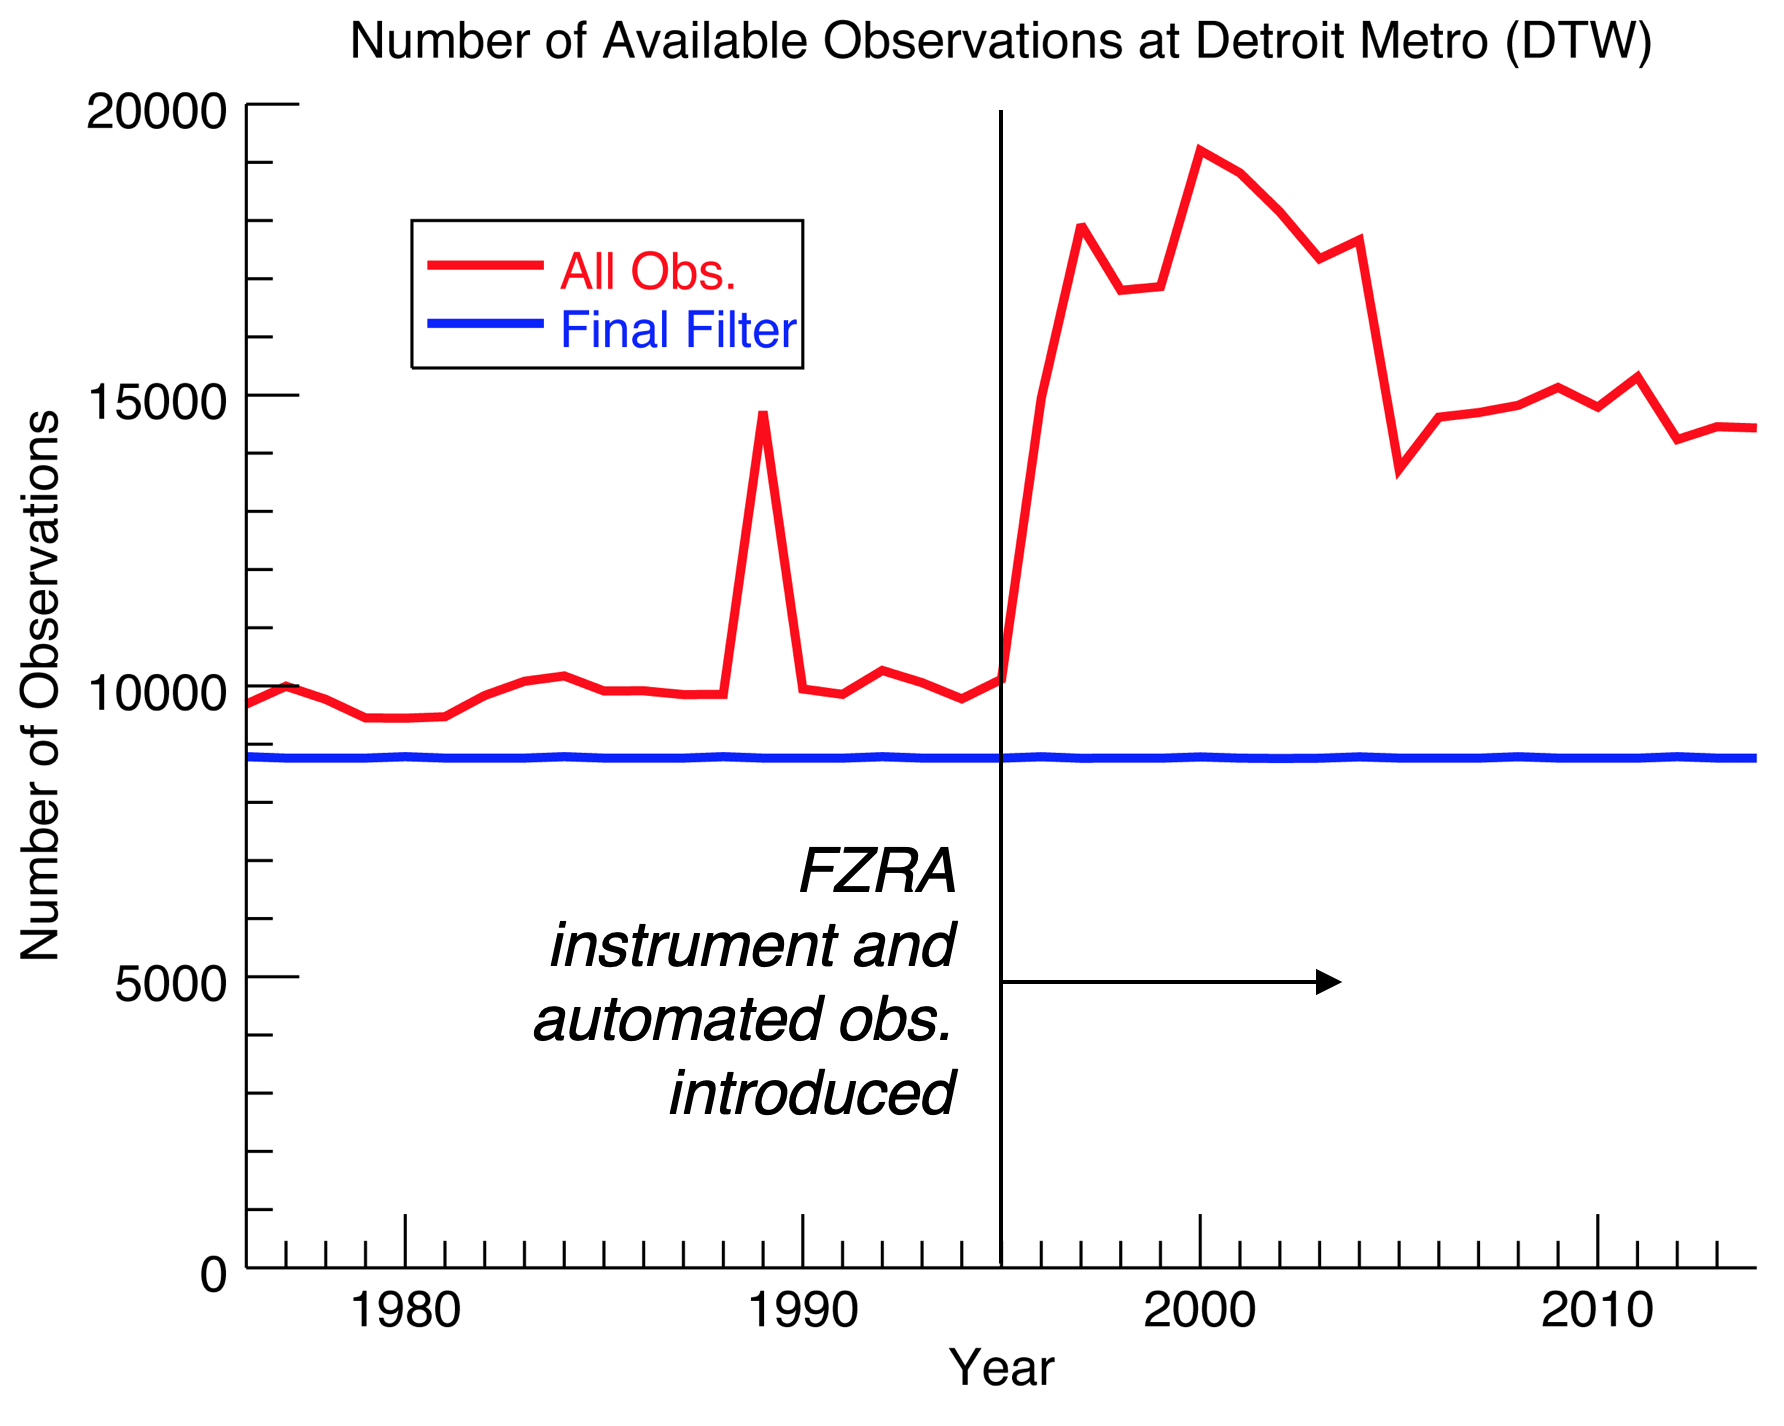
\includegraphics[width=0.5\textwidth]{Filtering_Plot.png}
\caption{\label{fig:filtering}Time series of total number of total observations per year at Detroit Metropolitan Airport before and after filtering to remove special observations and normalize the number of observations at each station to one per hour (i.e. 8760 per year or 8784 in leap years). Note: "FZRA" is referencing freezing rain by its METAR code.}
\end{figure}

\begin{figure*}
\centering
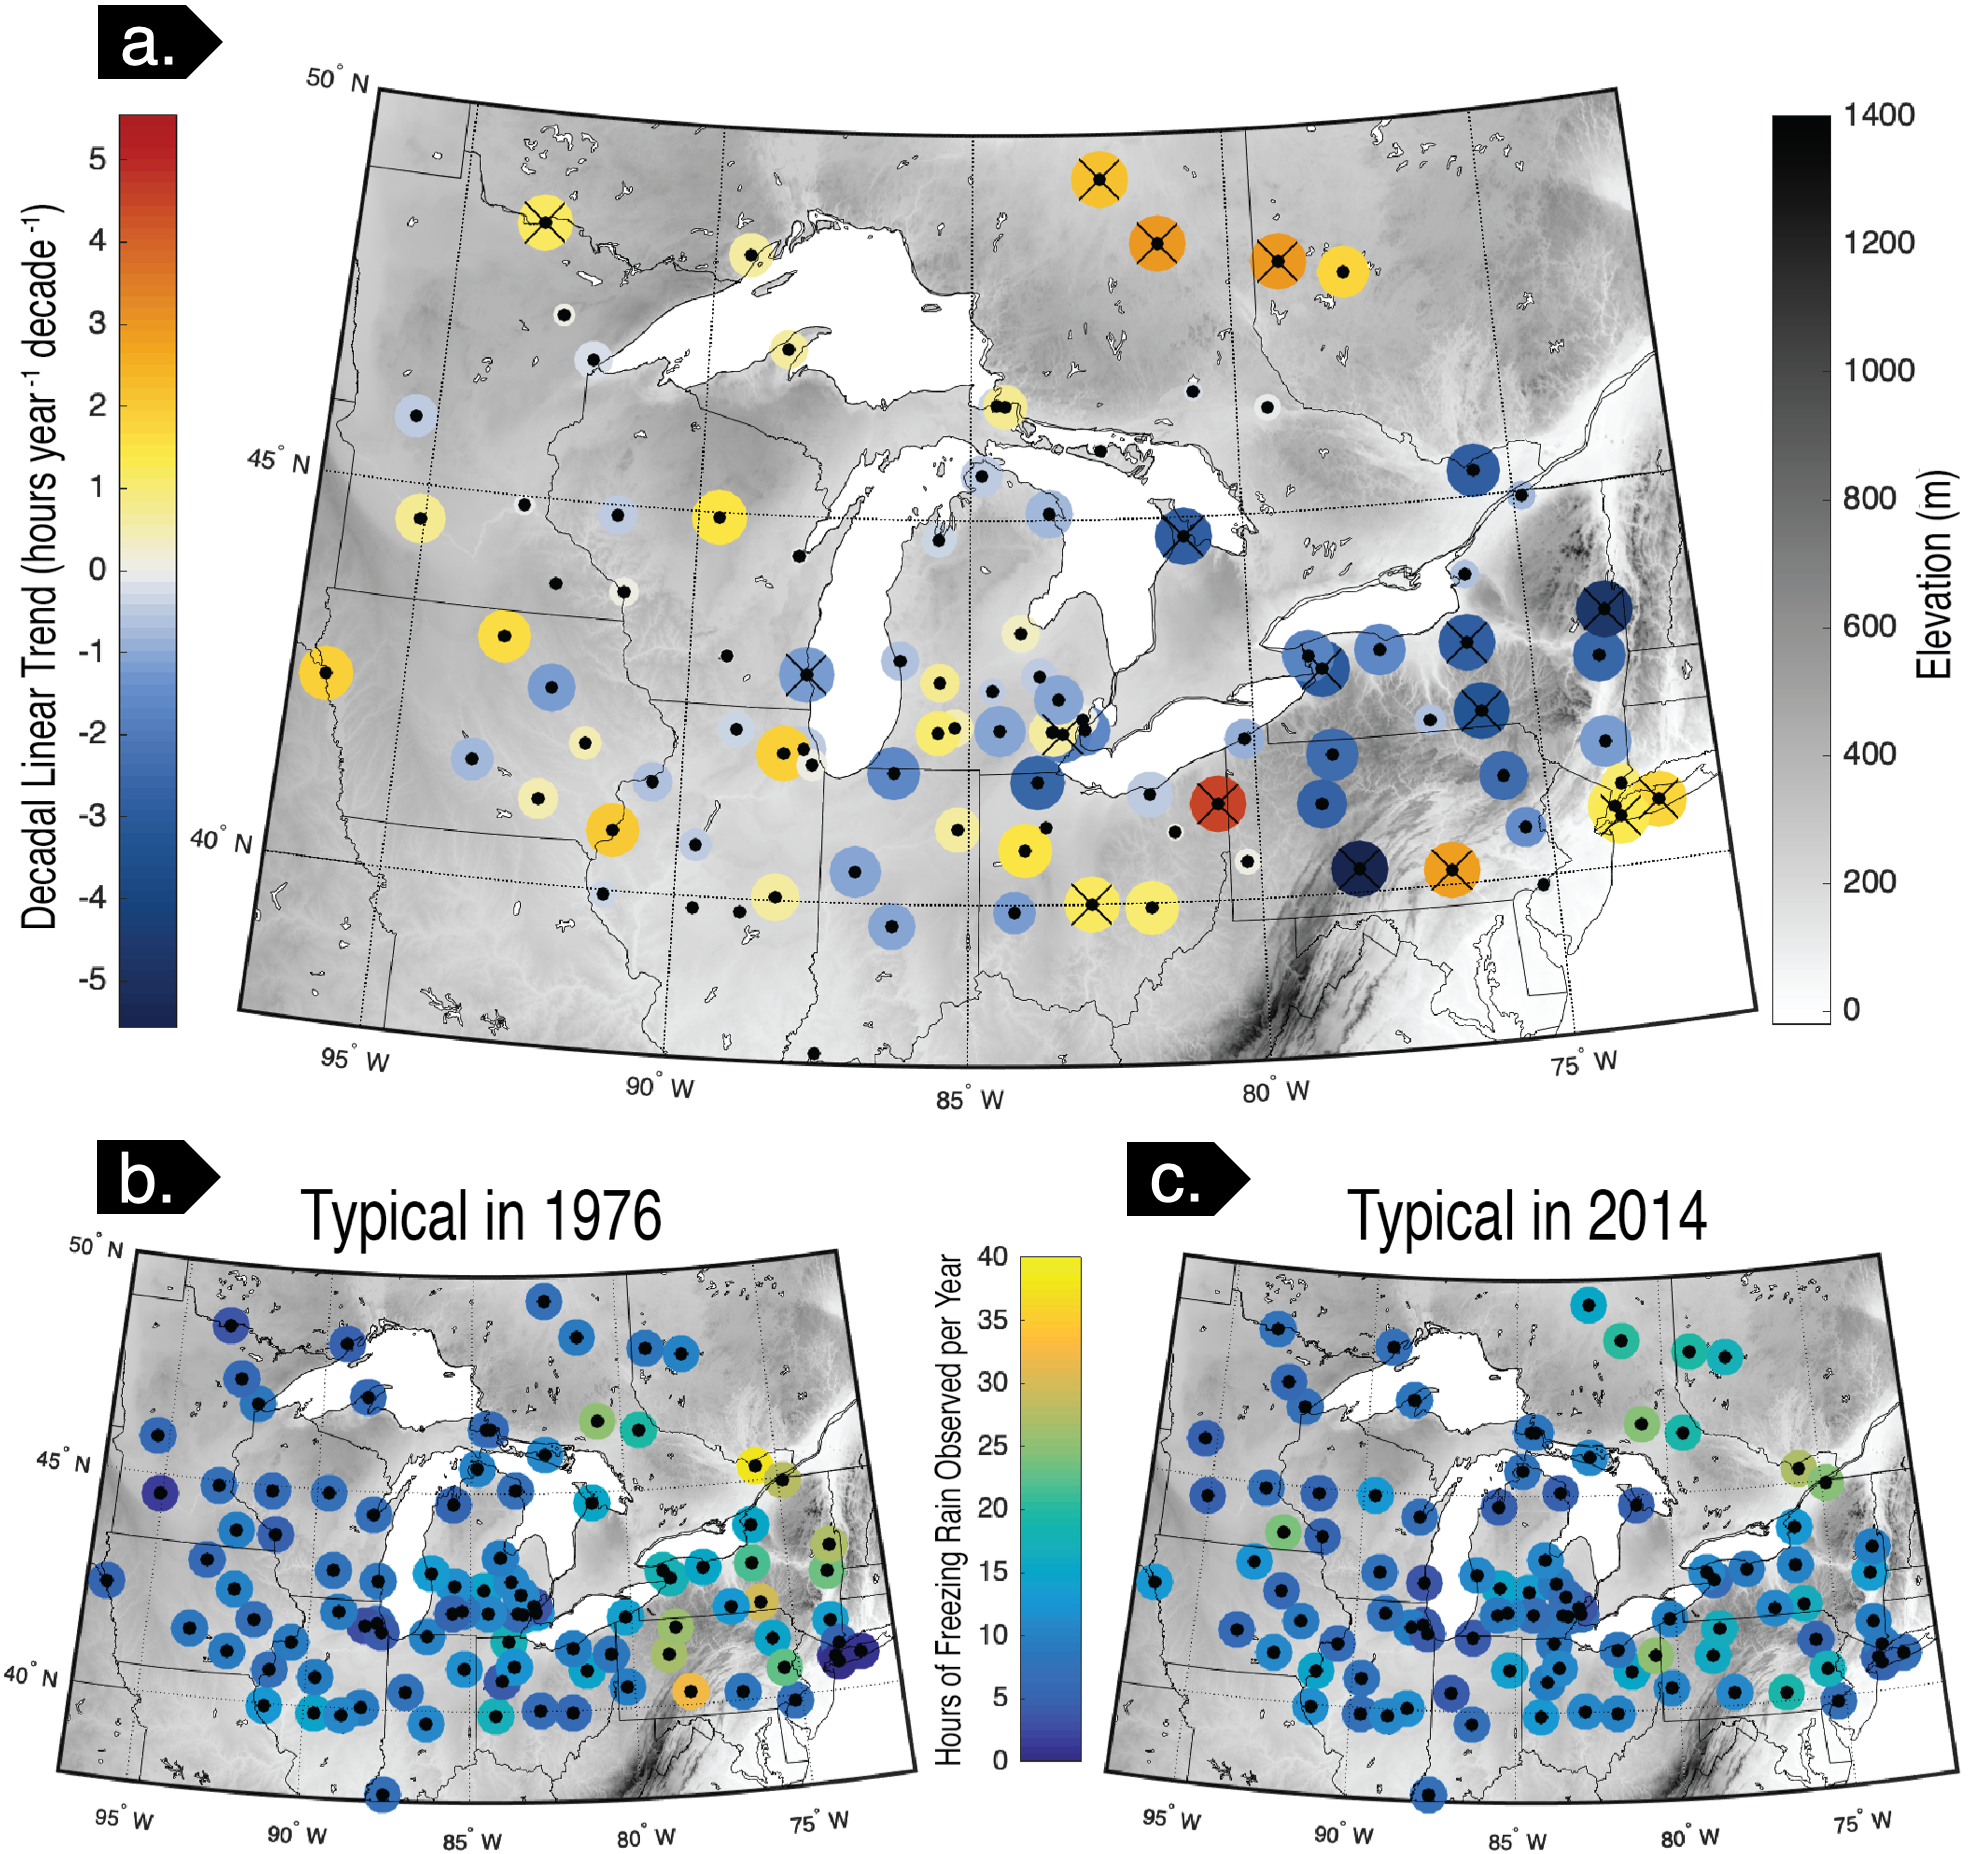
\includegraphics[width=1.0\textwidth]{FZRA_Trend_Maps.png}
\caption{\label{fig:trendmap}Elevation maps of the the Great Lakes region summarizing linear trends in total annual hours of freezing rain observed at each station from 1976 to 2014. De-noised or "typical" total annual hours of freezing rain calculated using the Theil-Sen slope estimation method are shown for first year (top left) and last year (top right) of the study period. Trends are depicted on a decadal scale at bottom. Filled circles at each observing station are scaled by $1 - p$ and Xs denote stations where the modified Mann-Kendall test indicates a monotonic trend at the $p<0.05$ level.}
\end{figure*}

\begin{figure*}
\centering
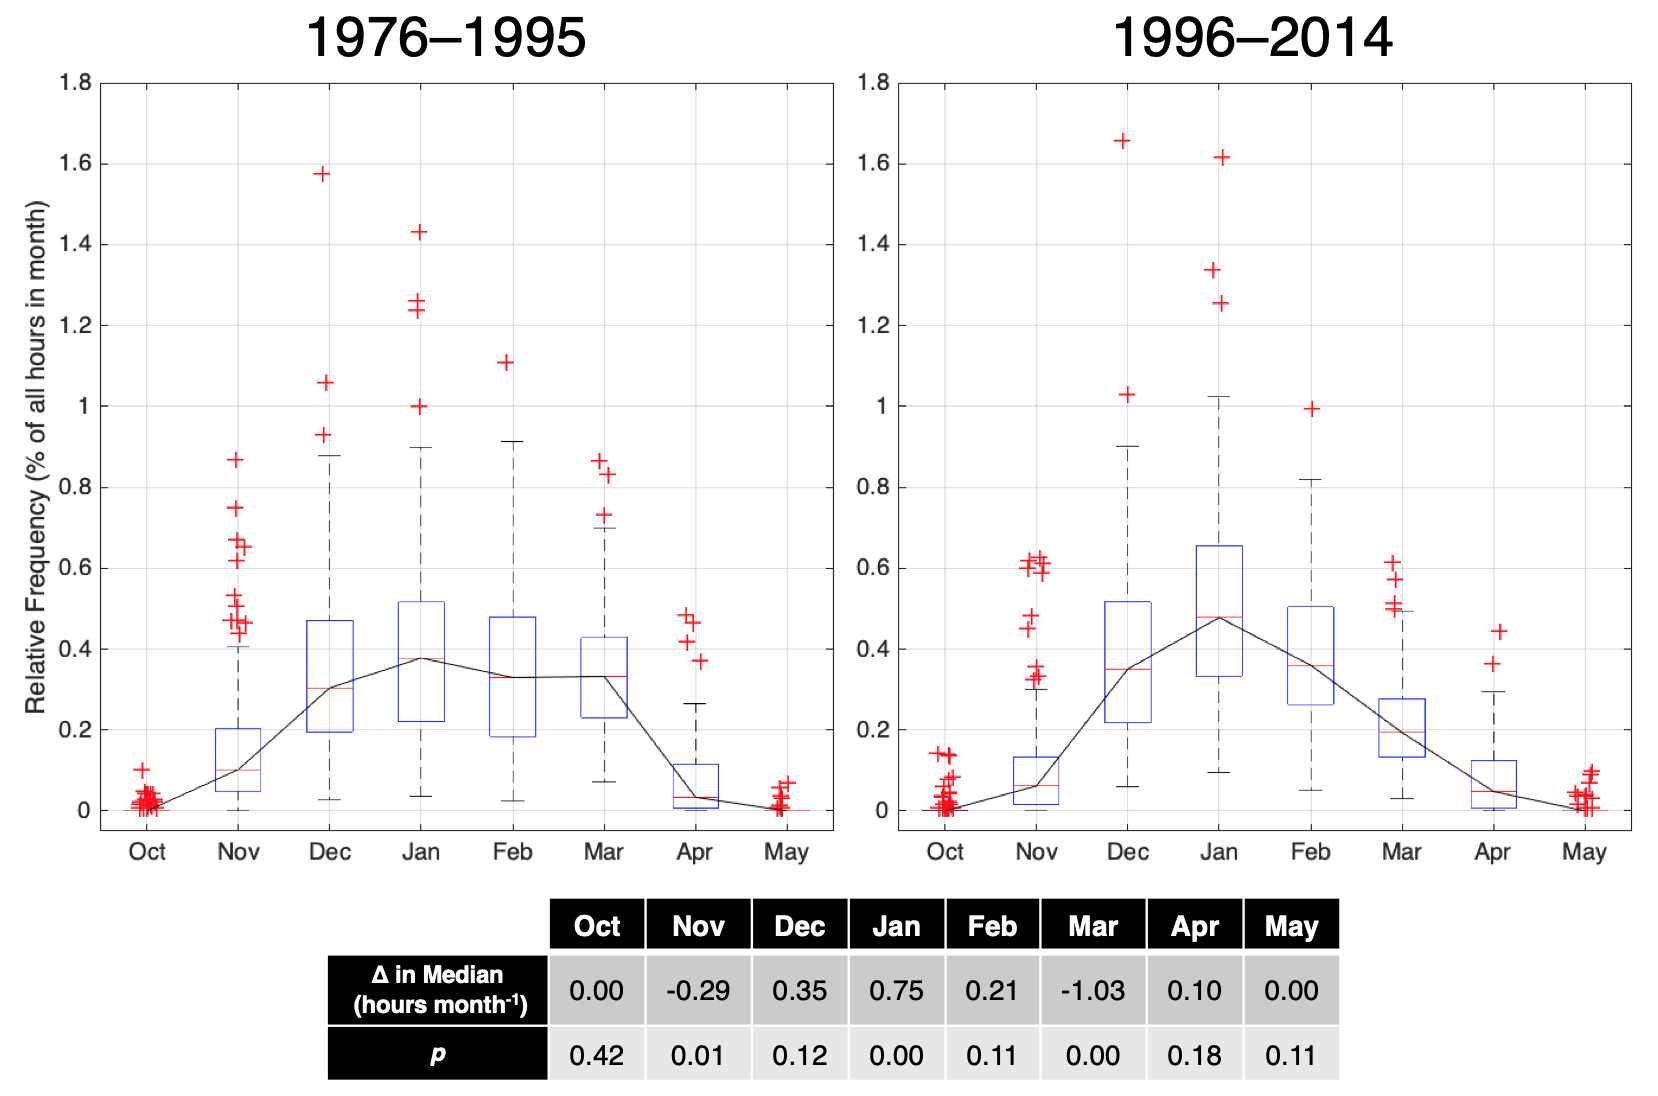
\includegraphics[width=1\textwidth]{Seasons_Boxplot.png}
\caption{\label{fig:seasonal} Comparison of seasonal frequency of freezing rain events between the first 21 years in the study period and the last 18 (to better coincide with the NARR-based dynamics analysis below). Red lines demarcate median values, boxes signify 25-75\% percentiles, whiskers inner fences, and red plus signs indicate outliers (jittered for visibility). Table lists $p$-values calculated using Mann-Whitney rank sum method to test for difference in median value.}
\end{figure*}
\todo[size=\small]{re: figure: add Mann-Whitney p-values in their own row.}

\begin{figure*}
\centering
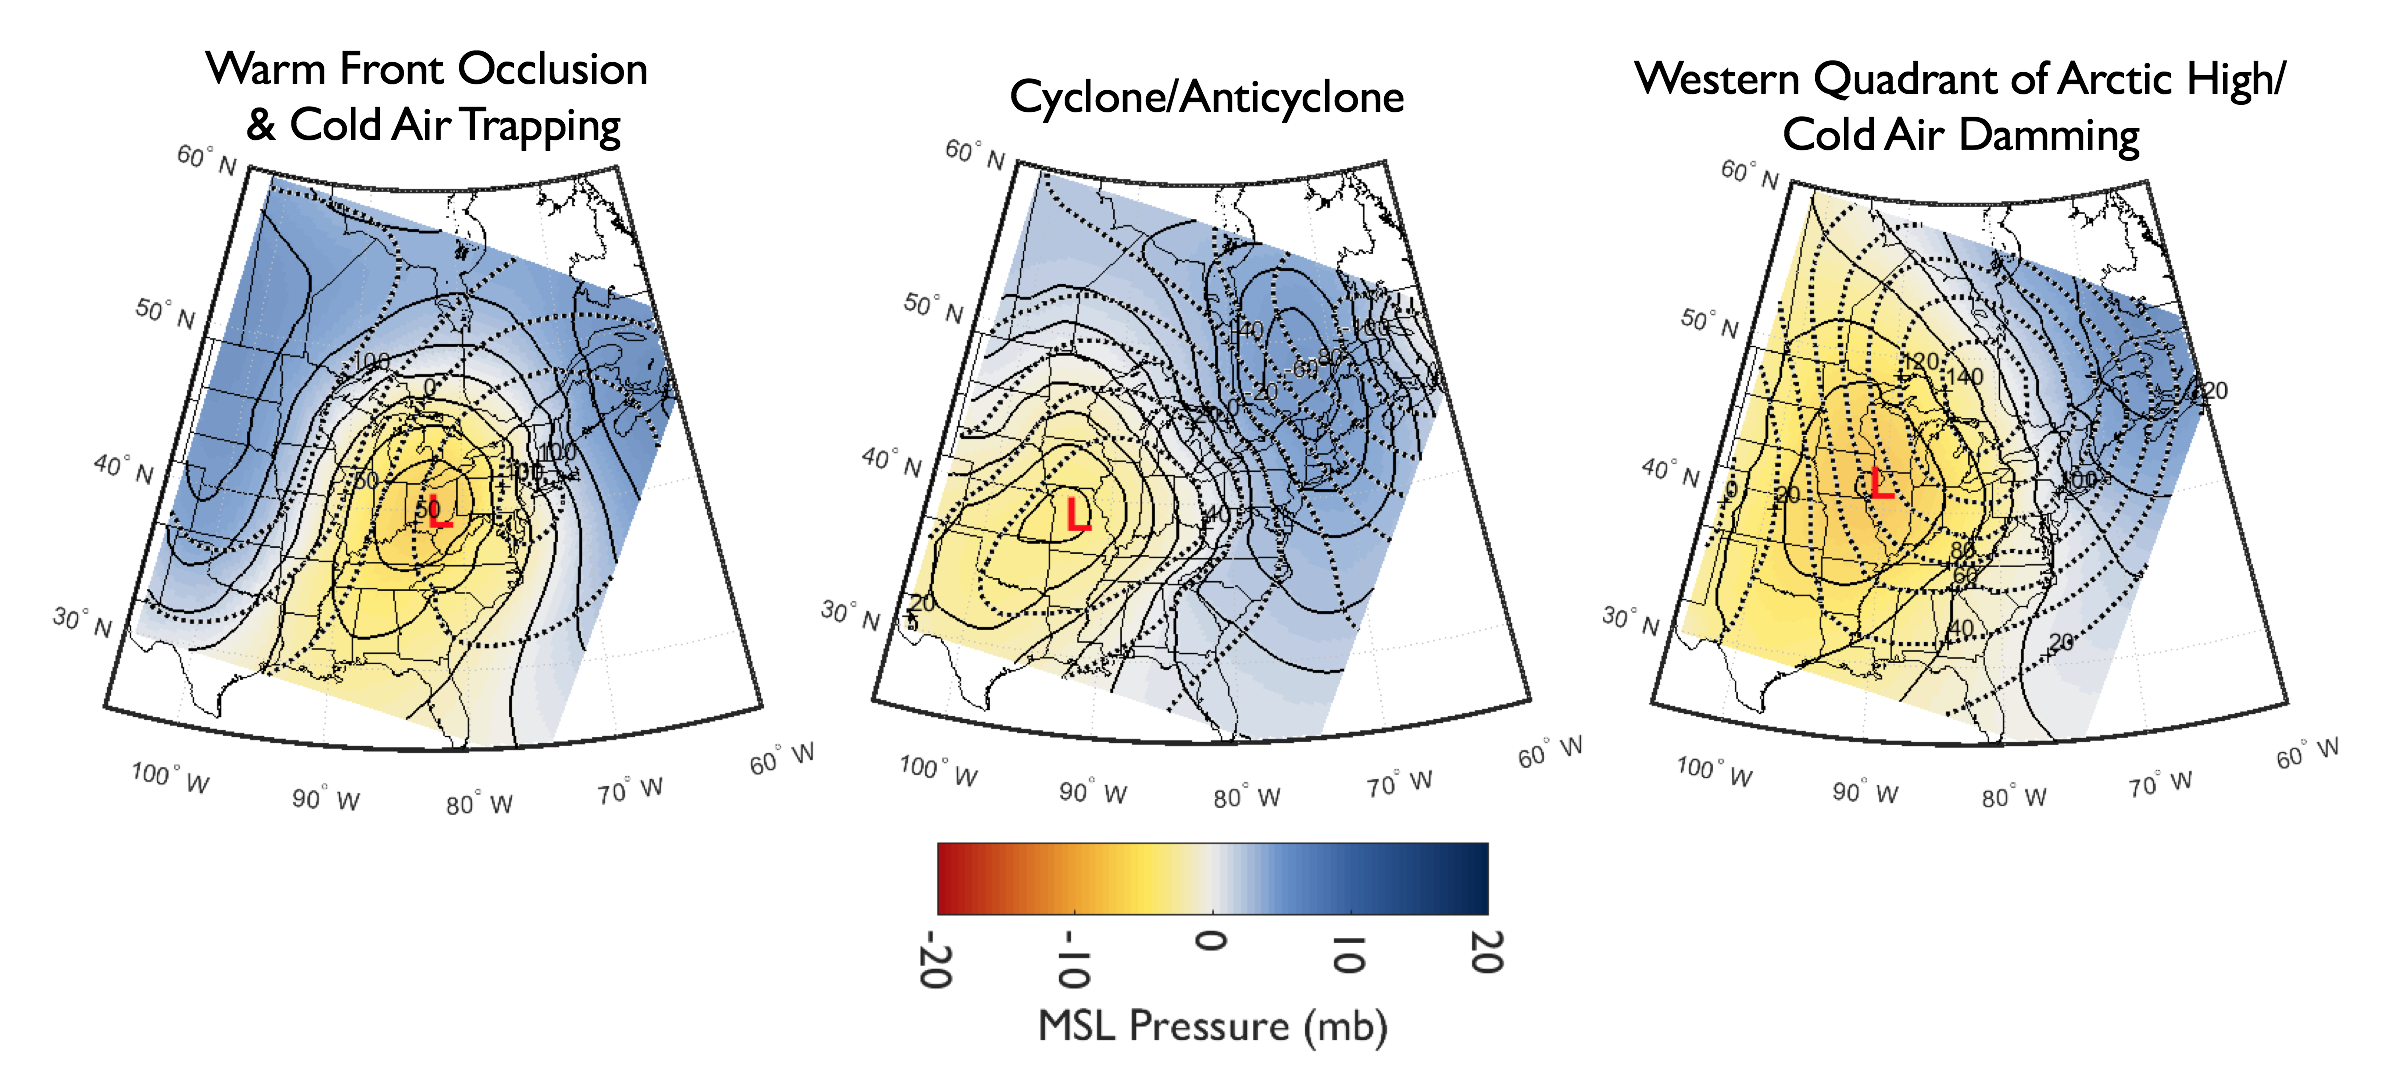
\includegraphics[width=1\textwidth]{Cluster_Centroids.png}
\caption{\label{fig:centroids} Centroid maps of cluster analysis  used to create three archetypal storm patterns. Solid lines refer to MSL pressure anomalies and dotted lines demarcate 850 mb geopotential height anomalies. Color bar shows anomalies, not absolute pressures.}
\end{figure*}

\begin{figure*}
\centering
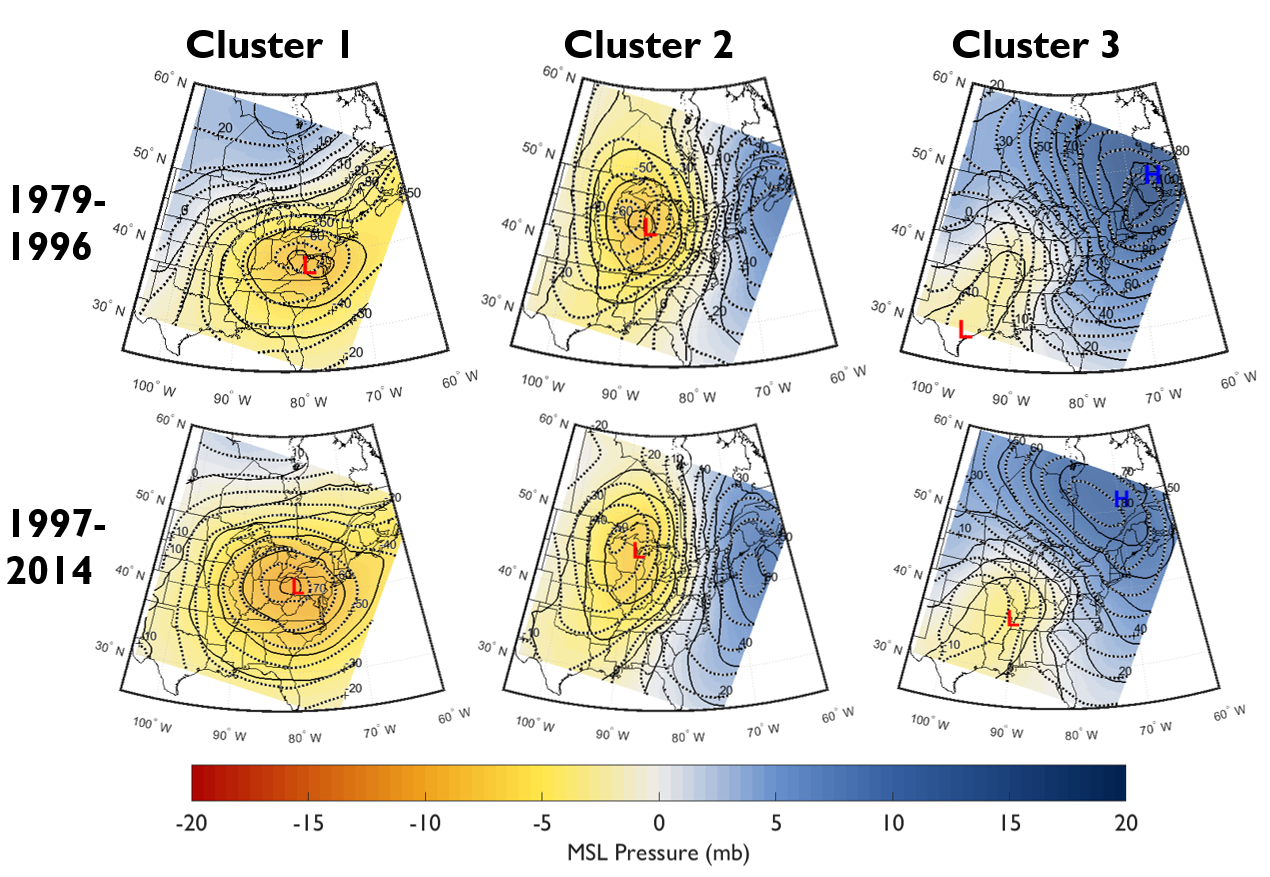
\includegraphics[width=\textwidth]{Clusters.PNG}
\caption{\label{fig:clusters} Freezing rain event archetypal patterns created using k-means algorithm with $k=3$. Color ramp and solid lines refer to MSL pressure anomalies in mb, while labeled dotted lines refer to 850 mb geopotential height anomalies in m.}
\end{figure*}

\begin{figure}
\centering
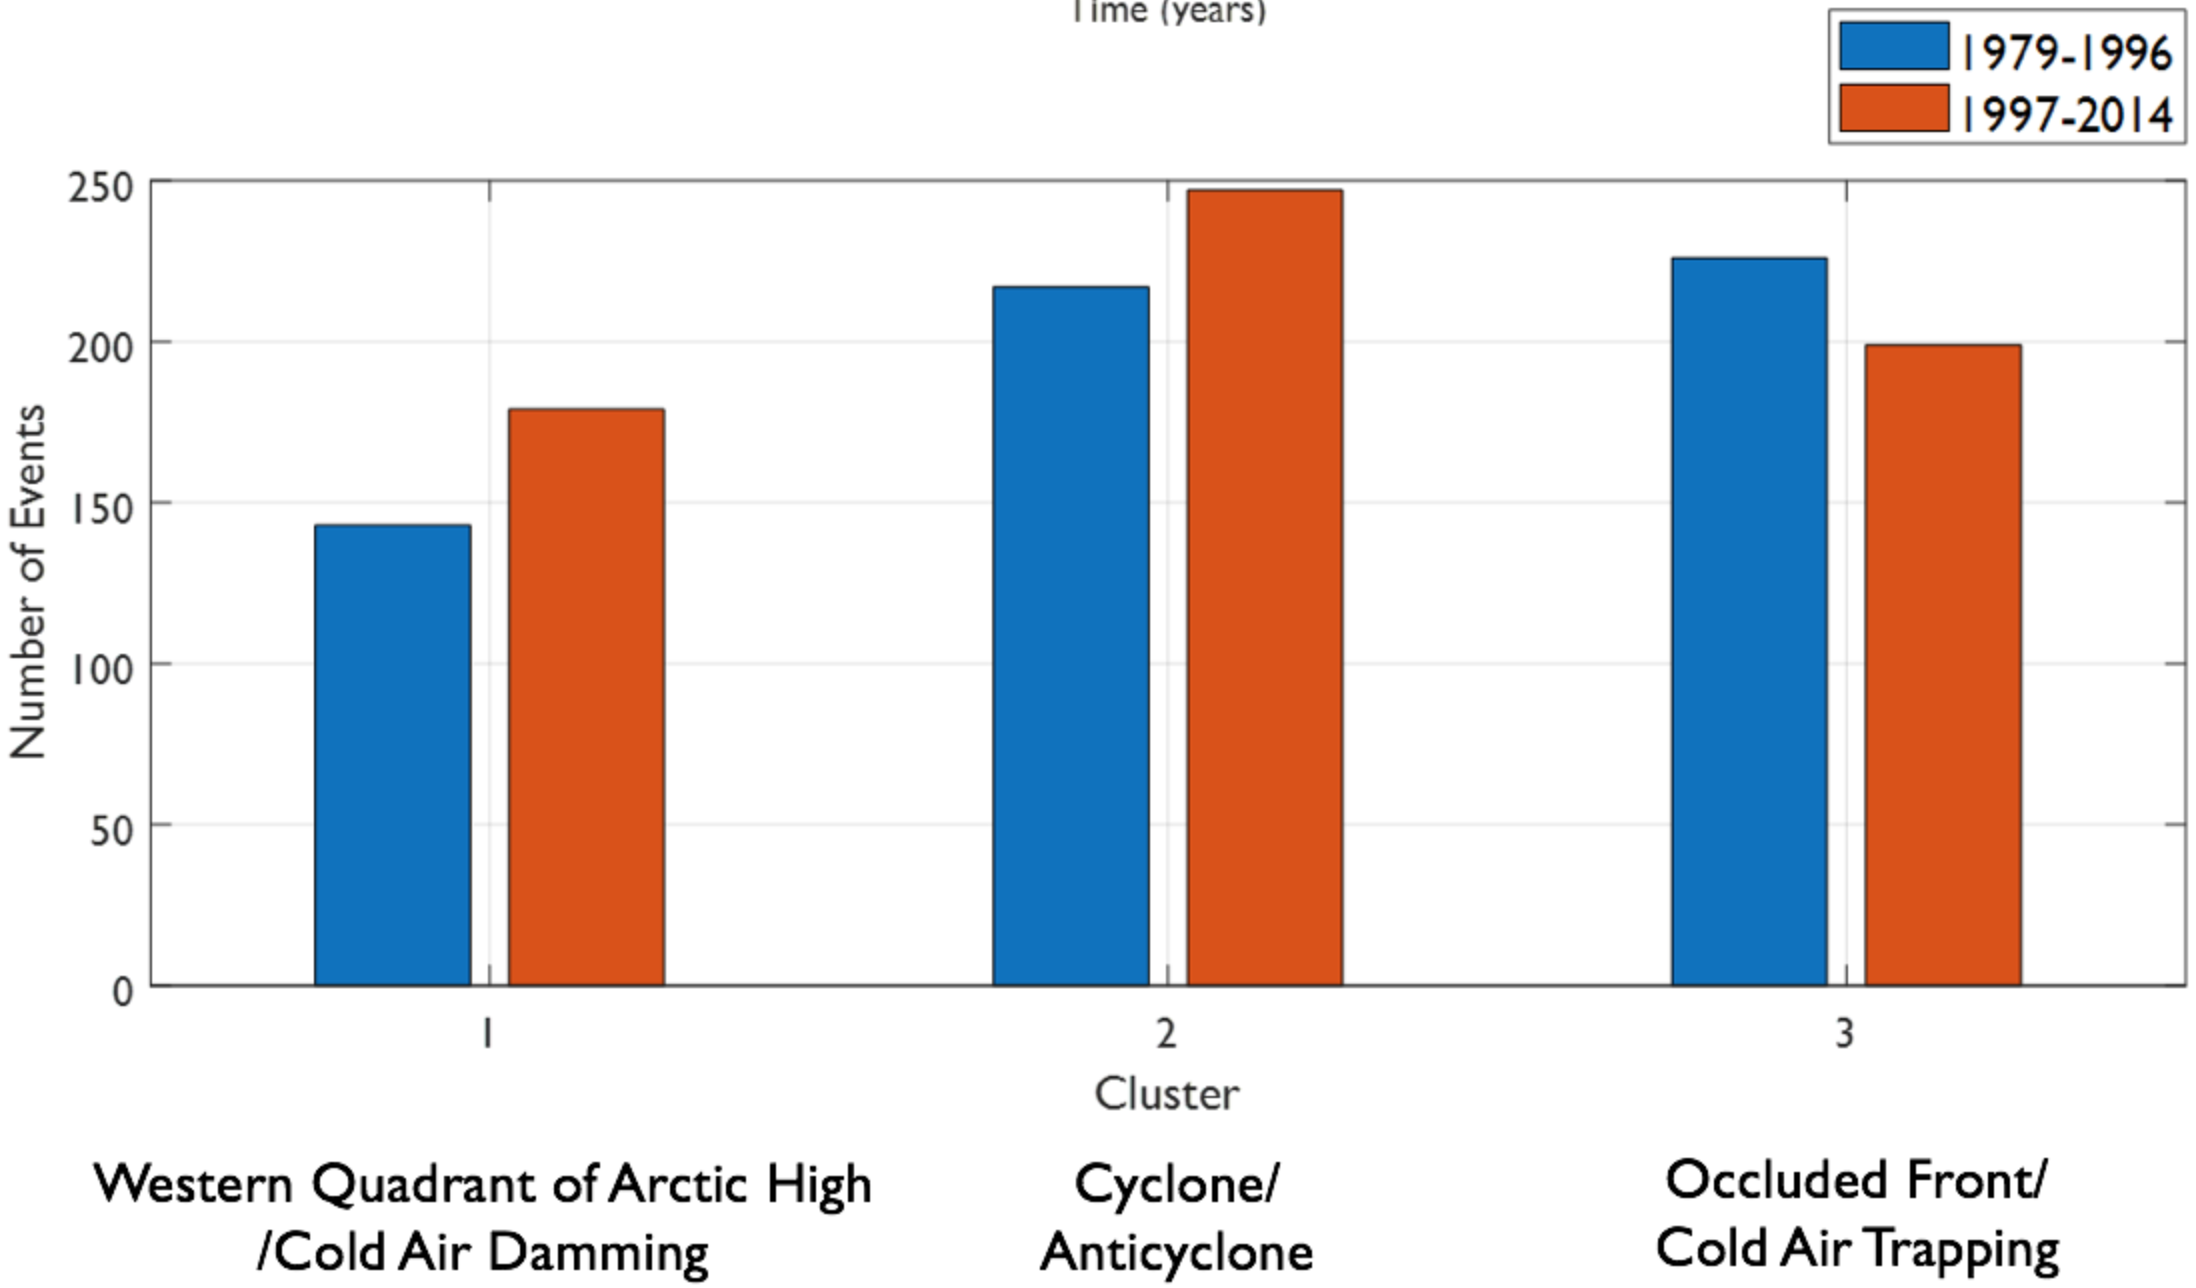
\includegraphics[width=0.5\textwidth]{Storm_Pattern_Change.png}
\caption{\label{fig:clusterchange} Timeline showing all events as classified into each of three clusters as calculated for the 1979--1996 period (top) and change in classification of events from the 1979--1996 period to the 1997--2014 period where the latter period is classified according to the centroids trained on the earlier period (bottom).}
\end{figure}

\end{document}

